
\documentclass[12pt]{report}
\usepackage{amsmath}
\usepackage{bm}
\usepackage{url}
\usepackage{graphicx} % Required for inserting images
\usepackage{placeins}
\usepackage{geometry}

 \geometry{
 a4paper,
 left=30mm,
 top=30mm,
 }

\usepackage{cite}
\usepackage{natbib}
\bibliographystyle{plainnat}

\title{SedSAT User's Manual}
\author{Arash Massoudieh
    \and
    Allen C. Gellis
    \and
    Cara L Peterman-Phipps }
\date{April 2023}
\renewcommand{\theequation}{\arabic{chapter}.\arabic{section}.\arabic{equation}}
\begin{document}

\maketitle

\section*{Executive Summary}
The Sediment Source Assessment Tool (SedSAT) User’s Manual provides comprehensive guidance for users of the SedSAT3 software, a tool developed for sediment source fingerprinting. The software facilitates the analysis of sediment sources and their contributions to a particular target site by utilizing elemental composition data. Key functions of SedSAT3 include data preparation, statistical analysis, and sediment source attribution using various methods such as Levenberg-Marquardt Maximum Likelihood Estimation, Genetic Algorithm Estimation, and Bayesian Inference. The manual outlines the steps required for importing and preparing raw data, followed by pre-analysis tasks like correlation matrix generation, outlier detection, and organic matter and particle size corrections. It also provides tools for advanced statistical analysis, including variance analysis and discriminant function analysis, to aid in selecting the most effective elements for fingerprinting. The manual culminates in detailed instructions for executing source attribution models and performing uncertainty analysis. A mathematical appendix explains the theoretical foundations for the modeling methods used in the software, offering users both practical and technical insights for sediment fingerprinting.
\tableofcontents




\chapter{Raw data preparation}
The raw data for SedSAT3 must be prepared as a single Excel spreadsheet file with multiple tabs. The first tab in the Excel file contains the elemental profiles of the target samples. The subsequent tabs contain the elemental profile for each source group. In each sheet, each row is assigned to one sample, the first column contains the names of samples, and each other column represents one element. In order for SedSAT3 to function, the data must be properly formatted (links to example datasets given in the example sample data file, downloaded from \url{https://sedsat.org/wp-content/Data/SampleData.xlsx}.). The specific text identifying column/field headers is unimportant, but the relative location of columns in the source and target datasets must be identical and is a core requirement for the program to run successfully. Column/field headers should be unique; no field name should match another field name within the same dataset. Note that each sheet must contain exactly the same elements named in exactly the same way. 


\section{Importing the data}\label{sec:importing_data}
To import the data, choose \textbf{File}$\rightarrow$\textbf{Import Data from Excel} from the menu bar located at the top left of the program, then navigate  to  the Excel file. 

Before the Excel file will be imported, you need to select the tabs you want SedSAT3 to import. 

When the Excel file is imported, a dialog box will appear asking you to identify the sheet that contains the target samples (Fig. \ref{fig:indicate_target_sample}). Select the radio button that corresponds to the target sample sheet, double-check that each subsequent Excel sheet is your source samples, and then select Ok. 

\begin{figure}[ht]\label{fig:indicate_target_sample}
    \centering
    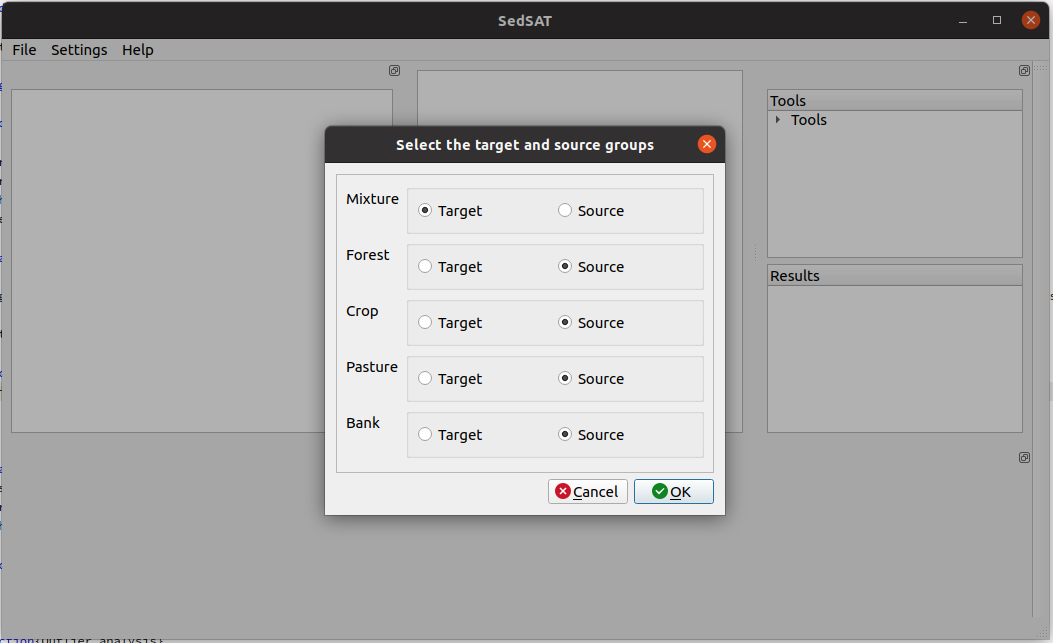
\includegraphics[width=14cm]{Figures/SelectSourceTargetGroups.png}
    \caption{Indicating the target sample}
    
\end{figure}


After identifying the target sample spreadsheet, a dialog box will appear to prepare for including/excluding samples, and then the constituent properties window will appear (Fig. \ref{fig:element_properties}.  Each window panel and individual columns can be resized by hovering your mouse between column headers; a double arrow will appear that allows the user to resize for better viewing.   

In the middle  window panel, there are five columns, the constituents are listed in the first column, and in the second column (Constituent Type), you can double-click on each constituent type to get a drop-down menu from the following list:

\begin{itemize}
    \item Element
    \item Isotope
    \item Particle size
    \item Organic carbon
    \item Exclude
\end{itemize}

Additionally, you can also exclude an element from the analysis by checking off the value in column five of the table. For isotopes, you need to choose the base element and the standard isotope ratio. This is needed for converting $\delta$ values to the elemental content of the isotope. For example, for $^{15}N$, the base element is $N$ and the standard isotope ratio is $(^{15}N/N)_{std}=0.003676$. If a constituent is indicated as particle size, organic matter, or excluded from the analysis, it will not be used directly for sediment fingerprinting.

You can always revisit the constituent properties through the top menu item \textbf{Settings}$\rightarrow$\textbf{Constituent properties} 

\begin{figure}[ht]
    \centering
    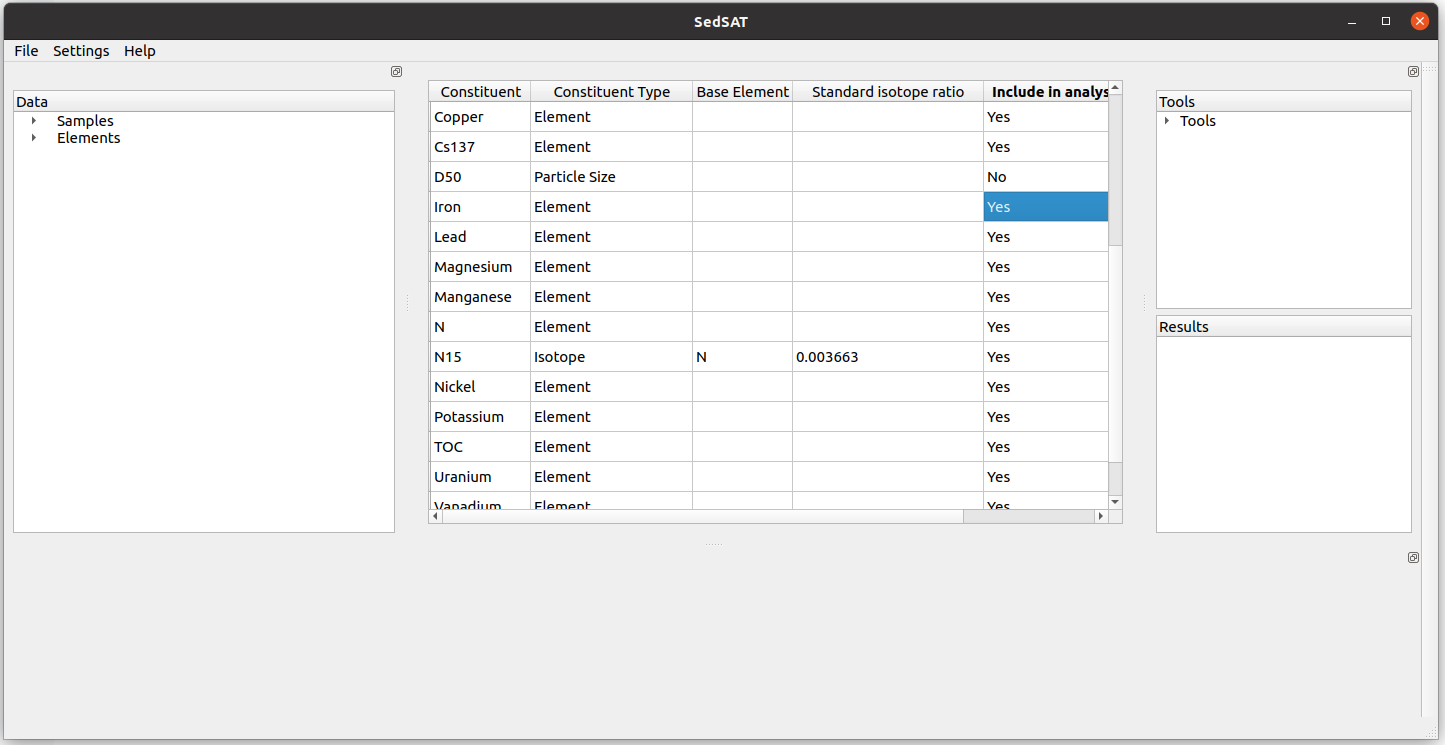
\includegraphics[width=14cm]{Figures/Element_Properties.png}
    \caption{Specifying Constituents' properties}
    \label{fig:element_properties}
\end{figure}

Now is a good time to save your project using \textbf{File}$\rightarrow$\textbf{Save} or pressing \textbf{CTLR+S}. The file will be saved in a readable JSON format with a file extension .cmb (CMB Source file). You can open it using any text editor and inspect the contents. You can load the project anytime in the future. 

You can visualize the elemental profiles using the tree view on the left side of the screen labeled data (Fig \ref{fig:constituents_vis}). 

\begin{figure}[ht]
    \centering
    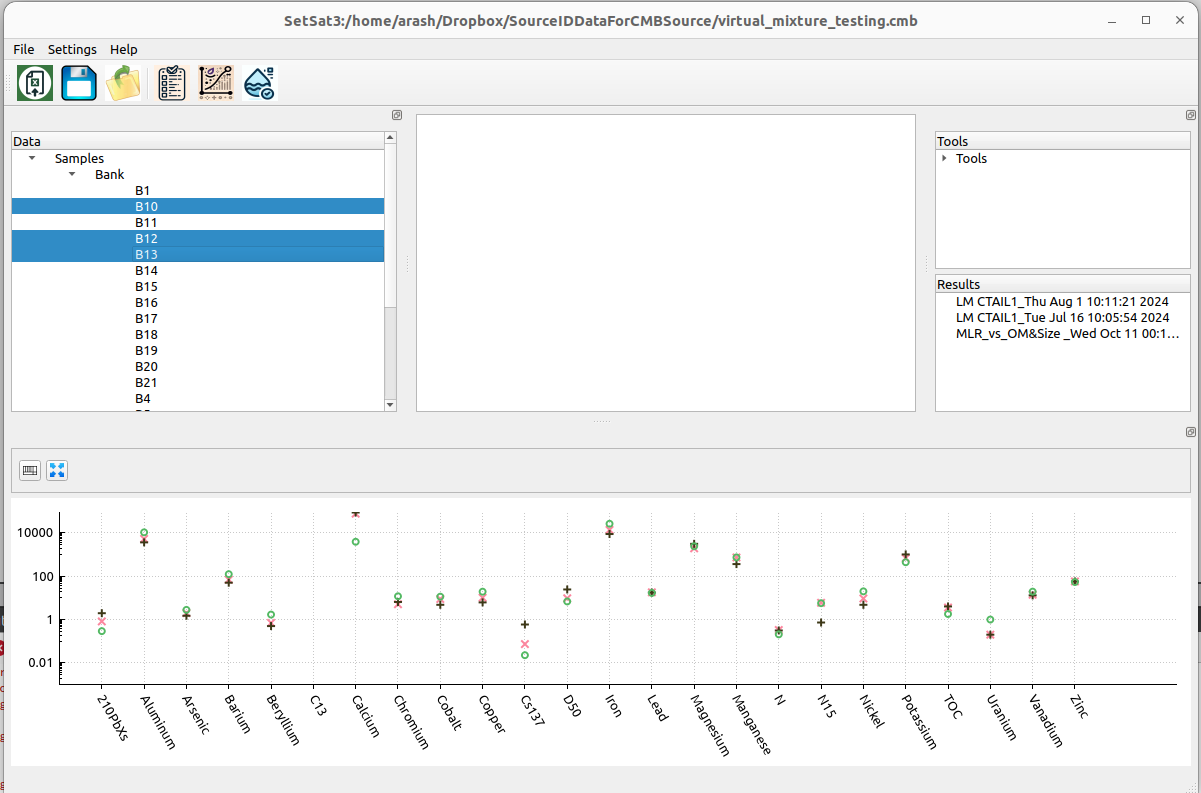
\includegraphics[width=14cm]{Figures/Constituent_Viz.png}
    \caption{Visualizing the raw data}
    \label{fig:constituents_vis}
\end{figure}

\subsubsection{Choosing samples to be discarded}



\chapter{Deterministic Fingerprinting tools}
This chapter outlines the complete sequence of steps and tools required to perform maximum-likelihood (deterministic) sediment fingerprinting. The process includes \textit{Outlier Analysis}, \textit{Organic Matter and Particle Size Correction}, \textit{Bracketing Analysis}, \textit{Stepwise Discriminant Function Analysis}, and concludes with the \textit{Fingerprinting} procedure.


\section{Outlier analysis}
The outlier analysis detects possible outliers in the elemental contents of individual samples. It first maps the concentration of each element in a source group using the Box-Cox transformation to the closest distribution to a Gaussian distribution. 

\begin{equation}
     \hat{y}_{i,j,k} = \begin{cases}
   \frac{\left(\frac{y_{i,j,k}}{\sigma_{i,j}}\right)^\lambda-1}{\lambda} & \text{for }\lambda \neq 0\\    
   log\left(\frac{y_{i,j,k}}{\sigma_{i,j}}\right) & \text{for } \lambda=0    
\end{cases}
\end{equation}

where $\sigma_{i,j}$ is the standard deviation of element $j$ in source group $i$.

The outlier analysis module first finds the optimal value of $\lambda$ that results in the closest transformed elemental concentrations to a normal distribution and then transforms the data using the optimal $\lambda$. The normality level is measured based on the Kolmogorov–Smirnov test. To view the optimal values of $\lambda$, use \textbf{Tools}$\rightarrow$\textbf{Other Statistical Tools}$\rightarrow$\textbf{Optimal Box-Cox parameters}.

After the Box-Cox transformation, the outlier analysis feature reports the deviation from the mean for each element in each sample of the selected source group. The deviation measure is calculated as:

\begin{equation}
    z = \frac{y_i-\mu}{\sigma}
\end{equation}

where $\mu$ and $\sigma$ are the mean and standard deviations of the transformed element content in the group. 

\textbf{The program will automatically run the outlier test when data is imported.} However, the user must go to Settings - Include/Exclude samples and in the Include column uncheck 'Yes'.  The outlier test uses a standard deviation of 3 as a default. To view samples that fail the outlier test the user can look at the Include/Exclude Samples tab.  In the Notes column, samples that have an element as an outlier are highlighted in red. Should the user want to change the standard deviation of the outlier test they will need to re-run the test using the directions below. 

To perform outlier analysis double-click on \textbf{Tools}$\rightarrow$\textbf{Pre-Analysis Tools}$\rightarrow$\textbf{2-Outlier Analysis}. From the form that appears, select the source group you would like the outlier analysis to be performed on. The threshold indicates the value which, if the absolute value of $z$ exceeds, the item will be highlighted in red. The default value of the threshold is 3, which means the elements outside of the 99\% bound will be highlighted in red. If you check the \textit{Use only selected elements} item, the Outlier Analysis will be generated only for the elements selected in \textbf{Settings}$\rightarrow$\textbf{Constituent properties}. Also, checking the \textit{Use only selected samples} checkbox only includes the samples that are selected in the analysis in \textbf{Settings}$\rightarrow$\textbf{Include/Exclude samples}.

Click the Ok button at the bottom of the form and then click on the table 
\includegraphics[width=0.5 cm]{Figures/table.png} on the window that appears. A table like Figure \ref{fig:outlier_table} will appear. The values outside of the specified threshold will be highlighted in red. 

At this point, if the user wants to remove a sample based on the outlier analysis, you must go to the left panel and select Settings, Include/Exclude samples and under the Include column, double click and check off the Sample.  It will appear as a 'No' (Fig. \ref{fig:include_exclude_samples}).

\begin{figure}[ht]
    \centering
    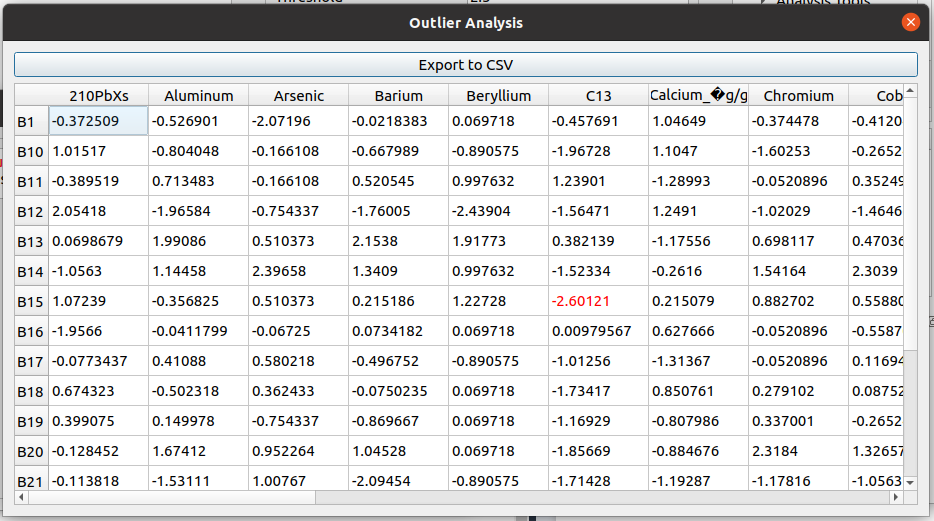
\includegraphics[width=10cm]{Figures/Outlier_table.png}
    \caption{Outlier table}
    \label{fig:outlier_table}
\end{figure}

\subsubsection{Choosing samples/elements to be discarded}
The user can decide which samples or constituents will be used in the sediment fingerprinting analysis based on the correlation, outlier, discriminant function, and bracketing analyses. To select the constituents to be included in the analysis from the top menu, choose \textbf{Settings}$\rightarrow$\textbf{Constituent Properties}. Follow the instructions in section \ref{sec:importing_data} to include or exclude constituents in the analysis. 
Choose \textbf{Settings}$\rightarrow$\textbf{Include/Exclude Samples} to exclude individual samples from the analysis. By clicking on this menu item, the program does the following: 

\begin{itemize}
    \item Performs outlier analysis on the source groups with a deviation threshold of 3.0 if it has not been done before. 
    \item Performs bracketing analysis on the target sample.
\end{itemize}

A window like Fig \ref{fig:include_exclude_samples} will appear. Select the source or target sample group from the top drop-down menu. Under the "Notes" column, the outlier and bracketing analysis results will be shown. The items that exceed the threshold given when outlier analysis was done or based on a default threshold of 3.0 if the outlier tool was not triggered before. Under the "Include" column, you can choose which samples to include or exclude in the analysis from this point on. 

\begin{figure}[ht]
    \centering
    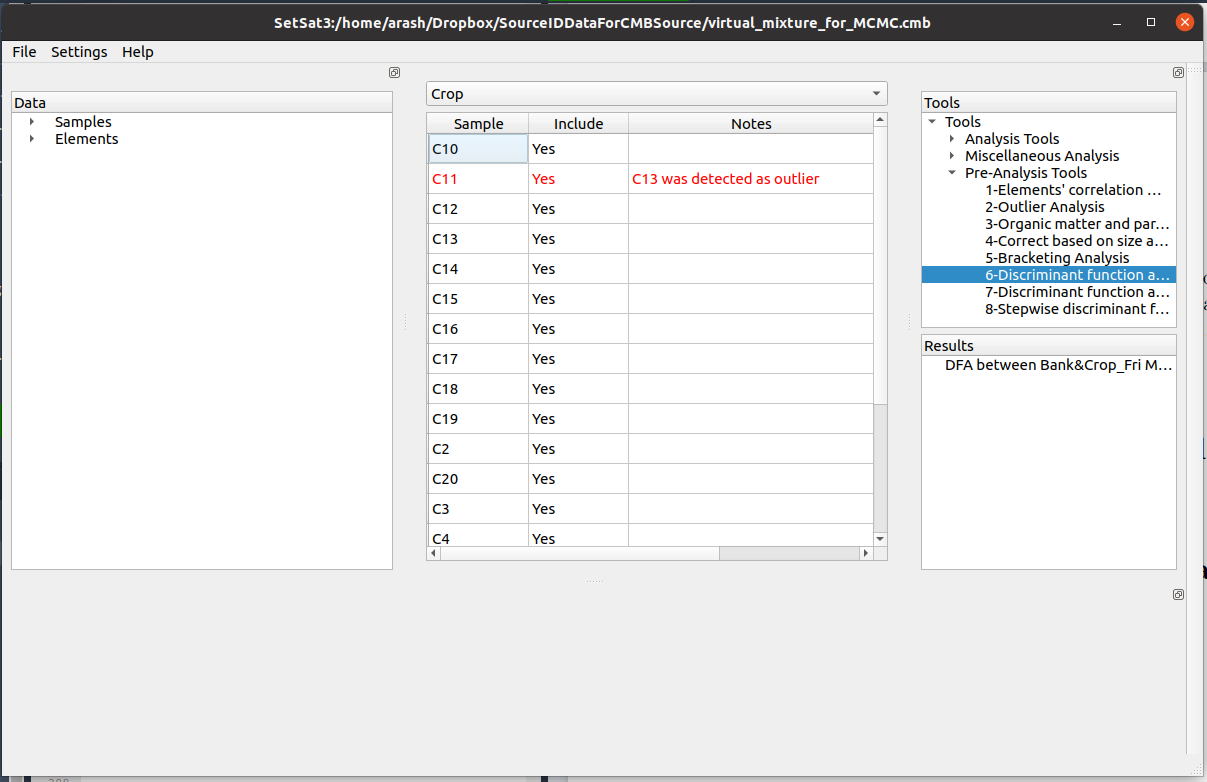
\includegraphics[width=14cm]{Figures/Include_Exclude_samples.png}
    \caption{Including or excluding samples from the analysis}
    \label{fig:include_exclude_samples}
\end{figure}
\FloatBarrier

\section{Organic matter and particle size correction}\label{sec:sizeandorganiccorrection}
In sediment source fingerprinting, organic matter, and size correction are important considerations when attempting to identify and apportion sediment sources within a watershed or catchment area. These corrections help account for the effects that different sediment sources, such as soil erosion, agricultural activities, or construction can have on an area and can vary in organic matter content and grain size distribution. Organic matter and size correction effectively account for the fact that the portion of particles mobilized from a source can have a different organic matter and size distribution than the samples collected to represent the source. A multiple linear or non-linear regression relationship between the elemental contents of different elements and the organic matter content and mean or effective size of the particles is performed. The relationship is then used to correct the source samples' elemental content based on the target samples' organic content and size. Note that this approach assumes that all sources contributing to the target sample are the same size and have the same organic content as the target sample. 

In SetSat3 two regression options are available: linear regression and a power-law regression: 

Linear regression: 
\begin{equation}
    y = a + \sum b_i e_i
\end{equation}

Power regression: 
\begin{equation}
    ln(y) = a + \sum b_i ln(e_i)
\end{equation}

where $a$ is the intercept, $b_i$ is the coefficient for the independent variable $i$ , and $e_i$ is the value of independent variable $i$. The independent variables can be particle size, organic matter content, or both. After the estimation of the regression coefficients and intercept, the corrected value of each element in each of the source samples is corrected as:

Linear regression:

\begin{equation}
    y_c = y + \sum b_i(e_{i,t} - e_{i,s})
\end{equation}

Power regression:

\begin{equation}
    y_c = y \prod \left(\frac{e_{i,t}}{e_{i,s}}\right)^{b_i}
\end{equation}

where $e_{i,t}$ is the value of independent variable $i$ in the target sample, and $e_{i,s}$ is the value of independent variable $i$ in the source sample.

\subsubsection{Performing Organic matter and  Particle Size Correction:}

In the tools window, click on \textbf{Tools}$\rightarrow$\textbf{Steps in Sediment Fingerprinting}$\rightarrow$\textbf{2-Organic Matter and Particle Size Correction}. 

Select the regression equation using the combo box labeled Equation, and the constituents representing organic matter and particle size on the form that appears. If the constituent representing organic matter or particle size is unavailable or you only want to correct based on one measure, leave the constituent for the dependent variable not to be used for correction blank. Click on the Ok button at the bottom of the form. The results window that appears contains the regression results for all of the constituents in all the sources. To visualize the regressions, click the graph button 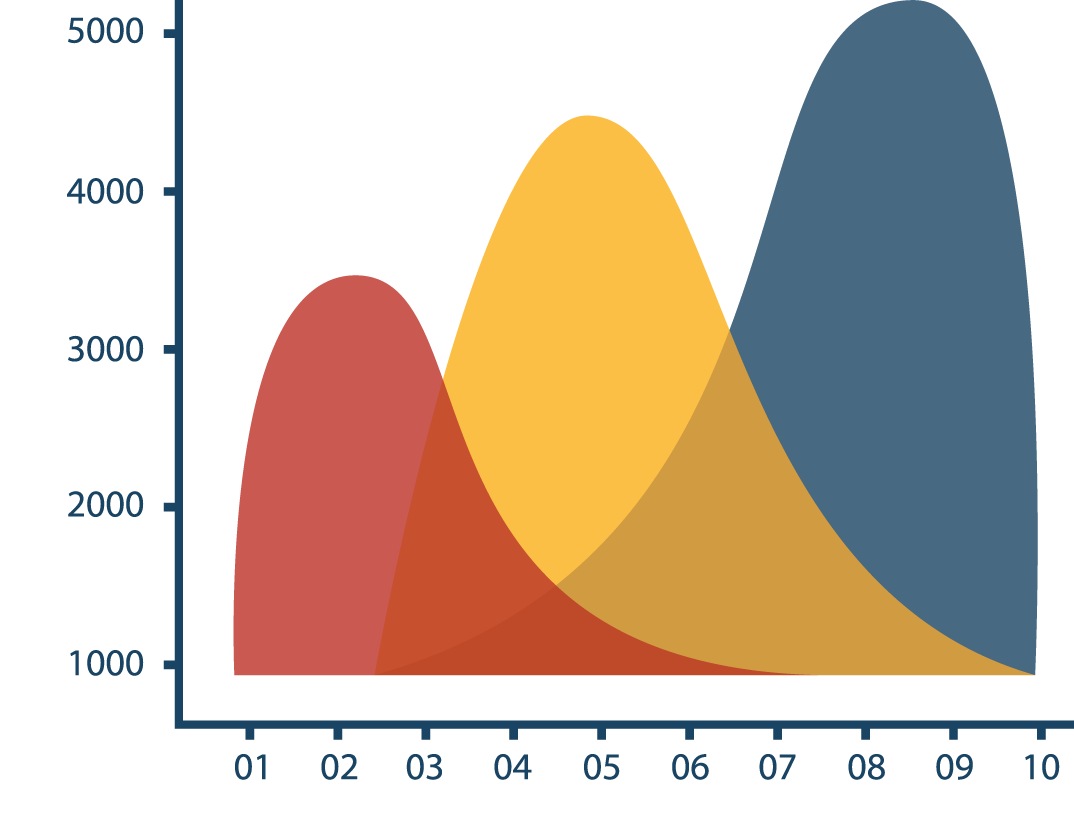
\includegraphics[width=0.5cm]{Figures/Graph.png}. A window like Fig. \ref{fig:regression_results} will appear. Select different constituents and independent variables from the combo boxes at the top. 

\begin{figure}[ht]
    \centering
    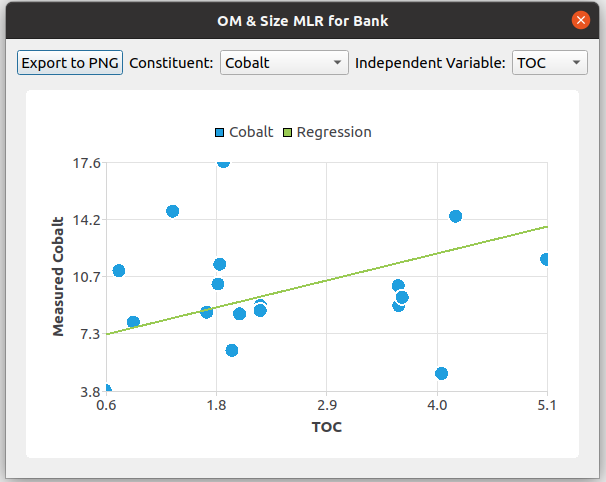
\includegraphics[width=10cm]{Figures/Regression_results.png}
    \caption{Graphical representation of OM and size correction regressions}
    \label{fig:regression_results}
\end{figure}
\FloatBarrier
To see the regression results in tabular form, click on the table button 
\includegraphics[width=0.5cm]{Figures/table.png} on the side of each source group in the results window. 

\begin{figure}[ht]
    \centering
    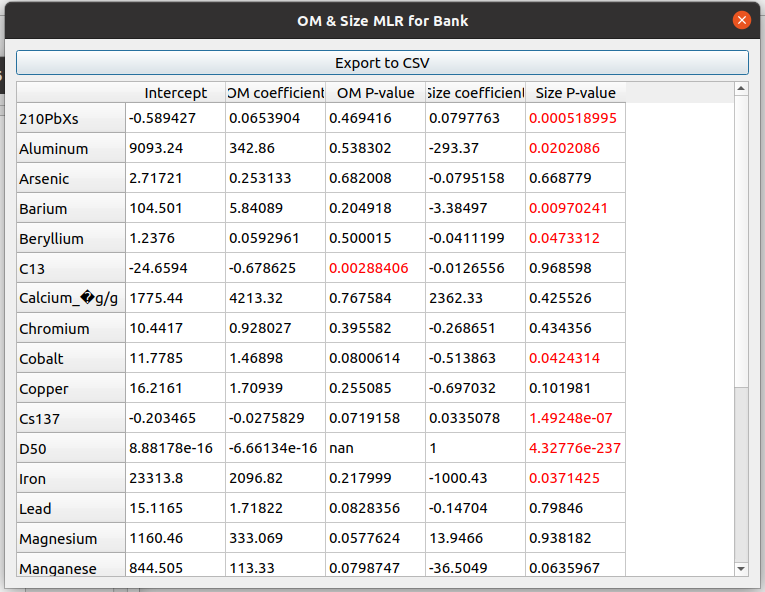
\includegraphics[width=9cm]{Figures/Regression_Tabular_results.png}
    \caption{OM and size correction results}
    \label{fig:regression_results}
\end{figure}
\FloatBarrier
The table contains the P-values that indicate the statistical significance of the OM and size. The p-values below 0.05 are in red.   

\subsubsection{Viewing the corrected elemental profiles}
Based on the p-values for the coefficients of OM and size, you can decide whether to correct based on each of those. From the top menu, left-hand side select \textbf{Settings}$\rightarrow$\textbf{Organic Matter and size correction}. A form including the regression results will appear as in figure \ref{fig:indicate_om_and_size_correction} will appear in the middle panel. 

\begin{figure}[ht]
    \centering
    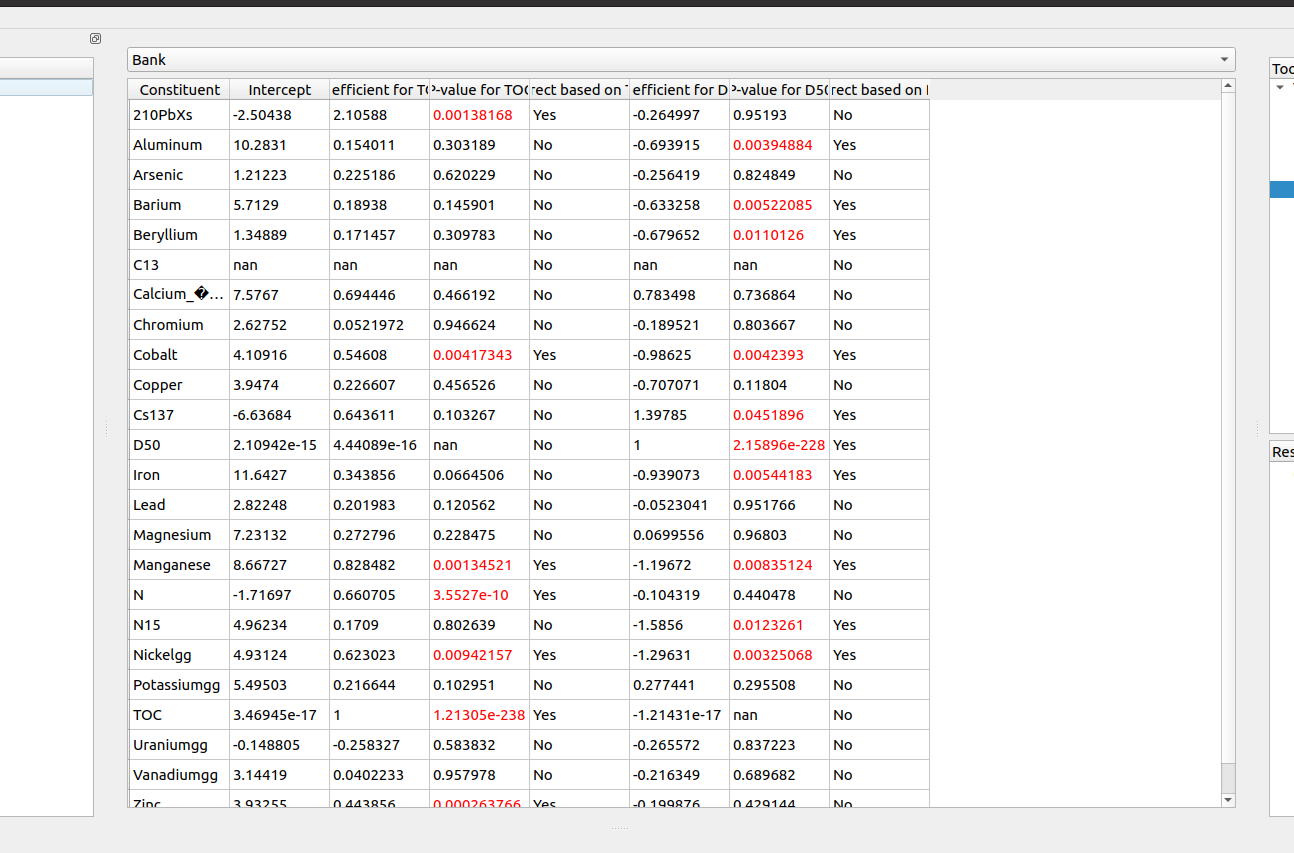
\includegraphics[width=12cm]{Figures/IndicateOMandSizeCorrection.png}
    \caption{Indicating OM and size correction}
    \label{fig:indicate_om_and_size_correction}
\end{figure}
\FloatBarrier
On the top combo box, you can navigate between various source groups. In the column titled P-value for TOC and the column titled P-value for D50, the p-values for the regression coefficients for organic matter and size are shown, respectively.  In column titled Correct based on TOC and column titled Correct based on D50, you can indicate whether to apply the corrections for particular elements based on organic matter and size. The items with a p-value of less than 0.05 are automatically selected to be applied.  

To view how the correction affects the elemental profiles of a particular source group based on a specific target sample from the tools panel, choose \textbf{Tools}$\rightarrow$\textbf{ 2 Organic Matter and Particle Size Correction}$\rightarrow$\textbf{ 2a Corrected results (after size and organic correction)}. In the form in the middle panel, choose the target sample on which you want the correction done. The results window that appears will contain panels for each of the source groups. To see the corrected elemental profiles of any source groups, click on the table button 
\includegraphics[width=0.5cm]{Figures/table.png} on the side of the panel (Fig. \ref{fig:corrected_elements_table}). 

\begin{figure}[ht]
    \centering
    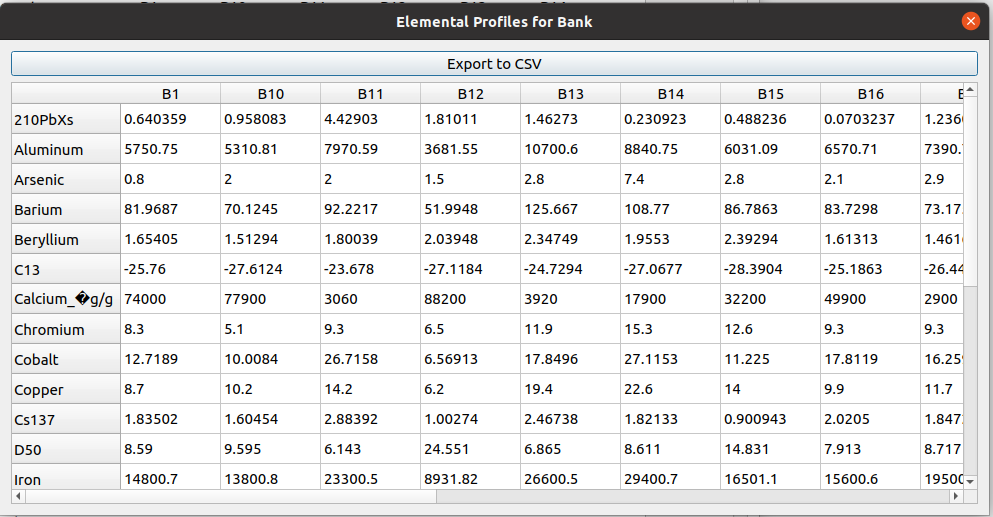
\includegraphics[width=10cm]{Figures/CorrectedEPsTable.png}
    \caption{Corrected elemental profiles based on size and organic matter}
    \label{fig:corrected_elements_table}
\end{figure}

\FloatBarrier
You can export the corrected elemental profiles to a CSV file to compare them with the original values. 

\section{Bracketing Analysis}

A bracketing analysis will check to see if there are elements in a target sample whose value is higher than all of the source samples. If the elemental content of a particular element in a target sample is higher than all source samples, no combination of source samples can reproduce an elemental profile close to the target sample. To perform bracketing analysis from the tools window, go to \textbf{Tools}$\rightarrow$\textbf{Steps in Sediment Fingerprinting}$\rightarrow$\textbf{3-Bracketing Analysis}. Select the target sample to be evaluated and press the Ok button. The results window indicates which elements passed and which did not pass the bracketing analysis. To see the results in tabular form or to export the result to a CSV file, click on the table button 
\includegraphics[width=0.5cm]{Figures/table.png}. 
To see the bracketing analysis result on all target samples from the top menu, choose \textbf{Settings}$\rightarrow$\textbf{Include/Exclude samples}. Choose the target group from the top drop-down menu at the top of the central form. The detailed results from the bracketing test indicates which element(s) violated the criteria for each sample and will be shown in the column titled "Notes" (Figure \ref{fig:bracketing_results}). 

\begin{figure}[ht]
    \centering
    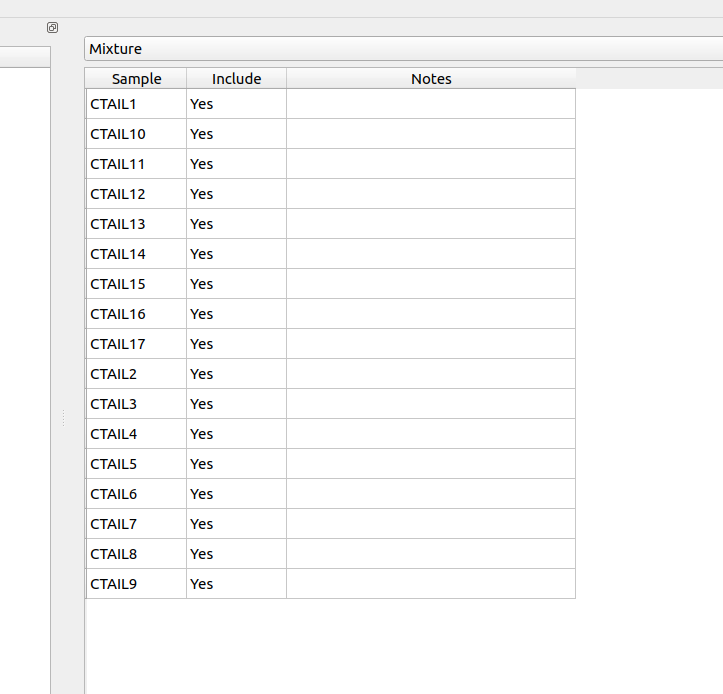
\includegraphics[width=10cm]{Figures/Bracketing.png}
    \caption{Bracketing test results}
    \label{fig:bracketing_results}
\end{figure}
\FloatBarrier

\subsection{Stepwise Discriminant Function Analysis (DFA)}
Discriminant function analysis (DFA) is a statistical technique used to predict the group membership of individuals or objects based on a set of predictor variables. It is a multivariate method that aims to find a linear combination of variables that maximally discriminate between two or more groups.

The primary goal of the DFA analysis is to determine a discriminant function that can effectively separate observations from different groups by reducing within-group variability and increasing between-group variability. In the context of sediment fingerprinting, DFA can be used to determine which elements most effectively differentiate between two or more sources. The linear discriminant function provides a scalar value which is calculated as a linear combination of the elemental contents for each sample: 


\begin{equation}\label{eq:discriminant_score}
    D(\tilde{\mathbf{y}}_k) = \mathbf{w}^T \tilde{\mathbf{y}}_k + c
\end{equation}

where $D(\tilde{\mathbf{y}}_k)$ is the discreminant score of sample $k$ , $\mathbf{w}$ is a vector of weights, $\tilde{\mathbf{y}}_k$ is the vector containing the elemental profile of a source sample $k$, and $c$ is a constant. 

SedSat3 uses Fisher's linear discriminant method \citep{fisher1936use}. The discriminant functions are found by solving an optimization problem that maximizes the Fisher criterion, which is the ratio of between-class variance to within-class variance. Mathematically, this is expressed as:

\begin{equation}
    J(\textbf{w}) = \frac{\textbf{w}^TS_b\textbf{w}}{\textbf{w}^TS_w\textbf{w}}
\end{equation}
    
where $S_b$ is the between-class scatter matrix, which measures the variance between the means of the groups, and $S_w$ is the within-class scatter matrix, which measures the variance within groups. 

This criterion is maximized by finding the eigenvectors of the matrix  $S_w^{-1} S_b$. The eigenvectors corresponding to the largest eigenvalues are the directions (weights) that define the discriminant functions.

\begin{equation}
    S_w^{-1}S_b \mathbf{w} = \lambda \mathbf{w}
\end{equation}

The weight vector is obtained as the eigenvector corresponding to the eigenvalue with the largest absolute value. 

Wilks' Lambda $\Lambda$ measures the ratio of within-group variability to total variability. The formula is:

\begin{equation}
    \Lambda = \frac{|S_w|}{|S_b+S_w|}
\end{equation}

The $\chi^2$ can be calculated as:

\begin{equation}
    \chi^2 = -\left(n-1-\frac{p+g}{2}\right)ln(\Lambda)
\end{equation}

with the degree of freedom  of $df = p\times(g-1)$.

where $n$ is the total number of samples in all source groups, $p$ is the total number of elements, and $g$ is the number of groups. 

An F-test can also be used to test the hypothesis that the centroids of discriminant scores (Eq. \ref{eq:discriminant_score}) of each group is the same. 

\section{Multi-way discriminant function analysis}

Multi-way DFA performs the discriminant analysis between all source groups holistically. It provides the test-statistics based on the weight vectors that will maximize the separation between all source groups. 

The results are similar to those for two-way and one-vs-the-rest stepwise discriminant function analysis (located in the 'Other Statistical Tools" menu), but here the statistics are calculated between the source group indicated and all other source samples. Figure \ref{fig:Chi2-DFA-multiway} shows the $\chi^2$ p-values.Significant tracers are selected one at time, beginning from the highest Chi-Squared p-value (left side of Fig. 4.7) to the lowest Chi-Squared p-value.  The graph indicates this as the tracers selection from C13 to N (fig. 4.7).

To see the separation as a result of selecting a certain set of elements, select \textbf{Tools}$\rightarrow$\textbf{Miscellaneous Analysis tools}$\rightarrow$\textbf{Discriminant Function Analysis (Mutliway)}. Check "Use only selected elements". Also indicate whether the Box-Cox transformation is to be conducted and whether the OM and size correction is to be performed before the analysis. Click on the "Ok" button. The result window contains three panels. The first panel shows the $\chi^2$ p-values for separation between the samples in each source from all the rest of the samples. A higher p-value indicates a lower separation between the source group and the rest.
Select the graph icon in the top panel to display the graph as shown in Figure 4.7; which shows the significant tracers.
\begin{figure}[ht]
    \centering
    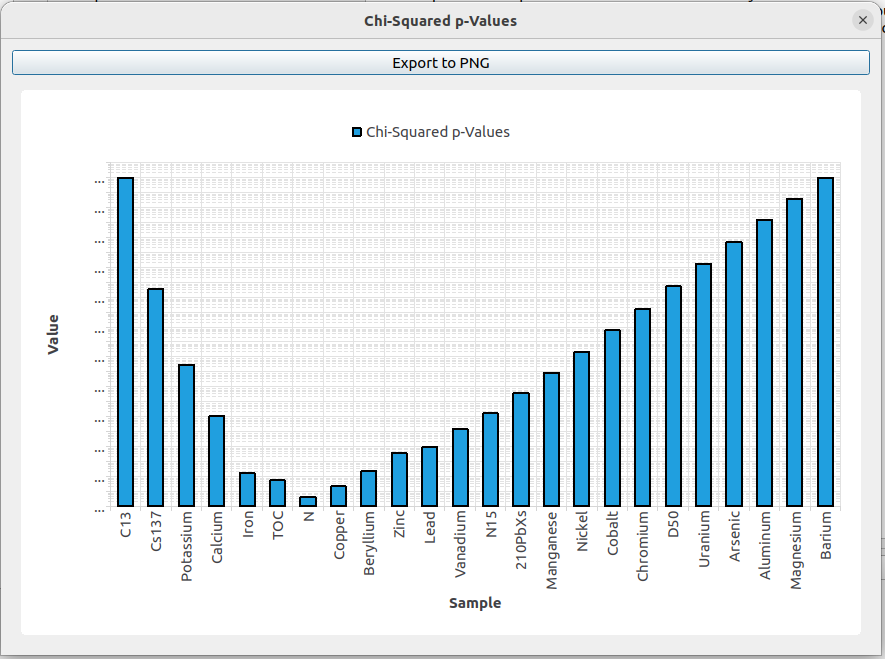
\includegraphics[width=14cm]{Figures/Chi2p-value-stepwise-multiway-DFA.png}
    \caption{$\chi^2$ p-values vs. the number of elements included for multi-way DFA}
    \label{fig:Chi2-DFA-multiway}
\end{figure}
\FloatBarrier

 Click on the table button 
\includegraphics[width=0.5cm]{Figures/table.png} on the side of any panel to see the values in tabular format (Fig. \ref{fig:Chi2-DFA-multiway-for-selected-elements}a). For example Fig. \ref{fig:Chi2-DFA-multiway-for-selected-elements}a shows a weaker separation between Pasture samples and the rest of the samples compared to other source groups. 

The second panel contains the F-test p-values. Click on Click on the table button 
\includegraphics[width=0.5cm]{Figures/table.png} on the side of the panel to see the values in tabular format (Fig. \ref{fig:Chi2-DFA-multiway-for-selected-elements}b). As it can be seen, the F-test p-values also indicate a weaker separation between pasture samples and other samples in this example. 

\begin{figure}[ht]
    \centering
    \begin{tabular}{c c}
        a) & b) \\
        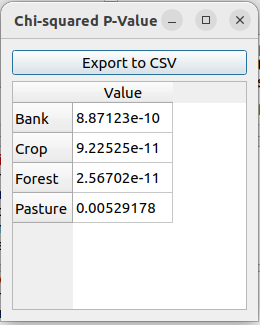
\includegraphics[width=6cm]{Figures/DFA-Multiway-Chi2-p-value-table.png} & 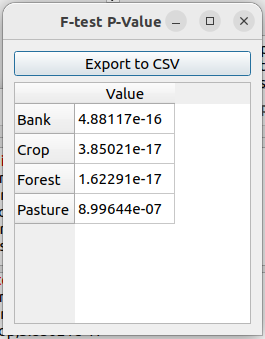
\includegraphics[width=6cm]{Figures/DFA-Multiway-F-test-p-value-table.png} 
    \end{tabular}
    
    \caption{a) $\chi^2$ p-values between each source group and the rest of samples for each source group b) F-test p-values between each source group and the rest of samples for each source group when Beryllium, $^{13}C$,  $^{137}Cs$, Manganese, N, Nickle, and Uranium are included in the analysis} 
    \label{fig:Chi2-DFA-multiway-for-selected-elements}
\end{figure}
\FloatBarrier

Panel three contains the discriminant scores based on the eigenvectors obtained for each source group. Click on the graph button 
\includegraphics[width=0.5cm]{Figures/table.png} on the side of the panel. Above the graph window that appears, select the two source groups the plot is intended to be shown for (Fig. \ref{fig:Multiway-DFA-scatter-plots}). The x-values show the discriminant scores based on the eigenvector maximizing the separation between the first selected source group and the rest of the samples while the y-values show the discriminant scores based on the eigenvectors obtained from the second selected source group.  

\begin{figure}[ht]
    \centering
    \begin{tabular}{c c}
        a) & b) \\
        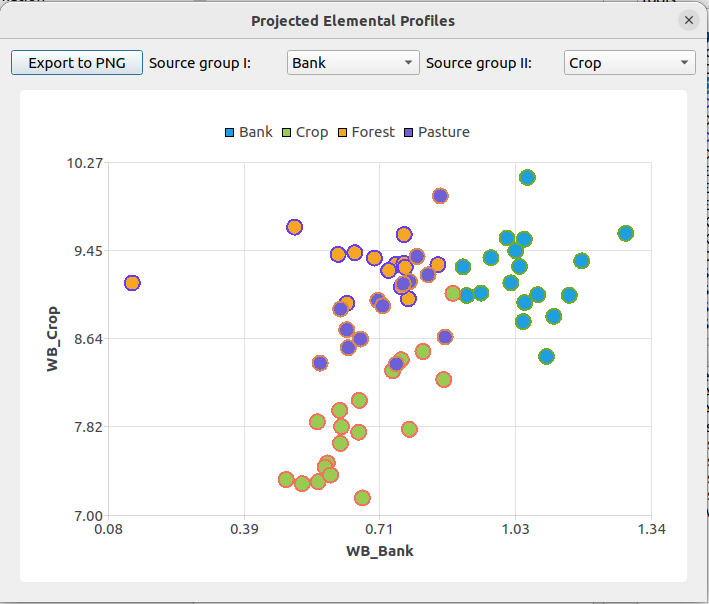
\includegraphics[width=7cm]{Figures/Multiway-Scatter-Bank-Crop.png} & 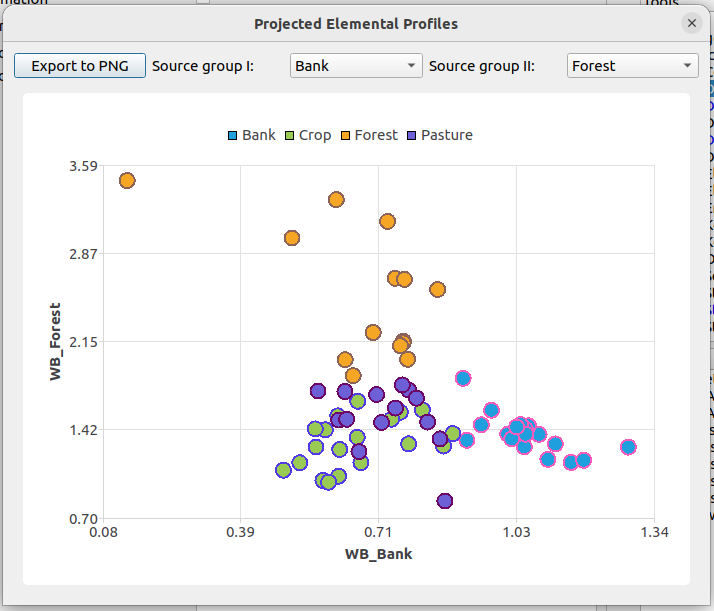
\includegraphics[width=7cm]{Figures/Multiway-Scatter-Bank-Forest.png} \\
        c) & d) \\
        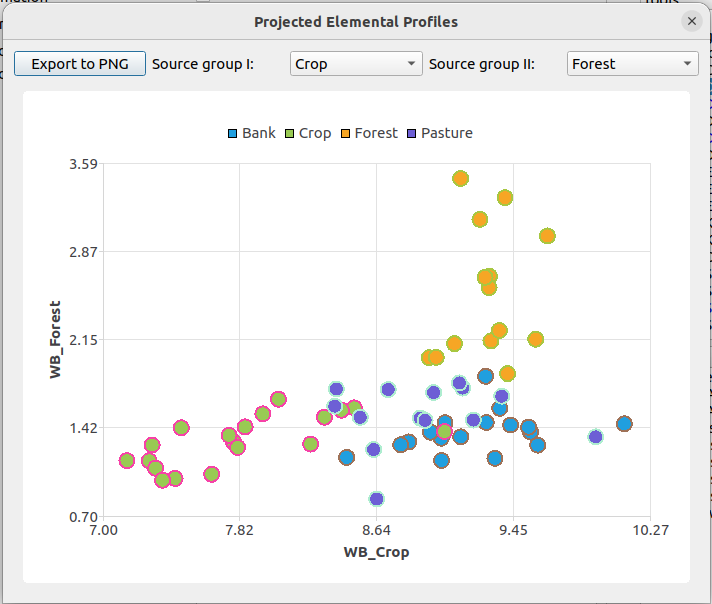
\includegraphics[width=7cm]{Figures/Multiway-Scatter-Crop-Forest.png} & 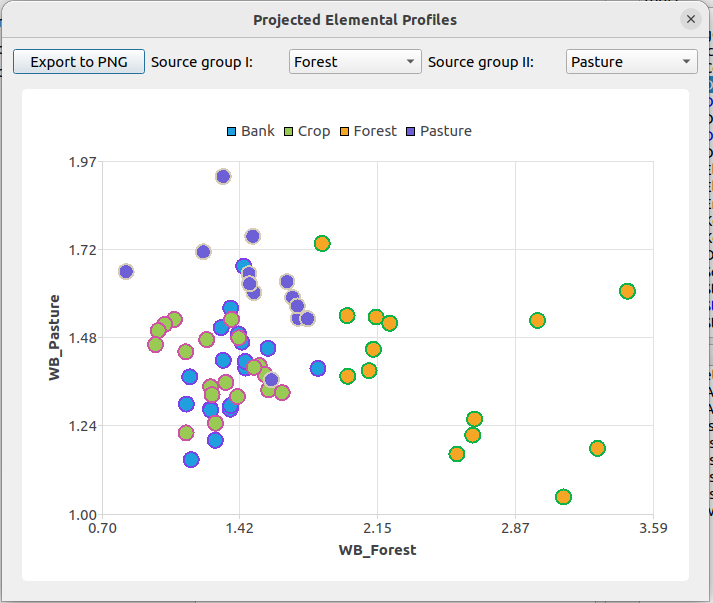
\includegraphics[width=7cm]{Figures/Multiway-Scatter-Forest-Pasture.png}
    \end{tabular}
    
    \caption{Scatter plots showing discriminant scores based on the eigenvectors obtained from a) Bank and Crop, b) Bank and Forest, c) Crop and Forest, and d) Forest and Pasture} 
    \label{fig:Multiway-DFA-scatter-plots}
\end{figure}
\FloatBarrier

Finally, the forth panel contains the eigenvectors obtained based on maximizing the separation between each source groups and the rest. Click on the table button on the side of the panel to see the eigenvectors in tabular form (Fig. \ref{fig:Multiway-eigenvectors}). 

\begin{figure}[ht]
    \centering
    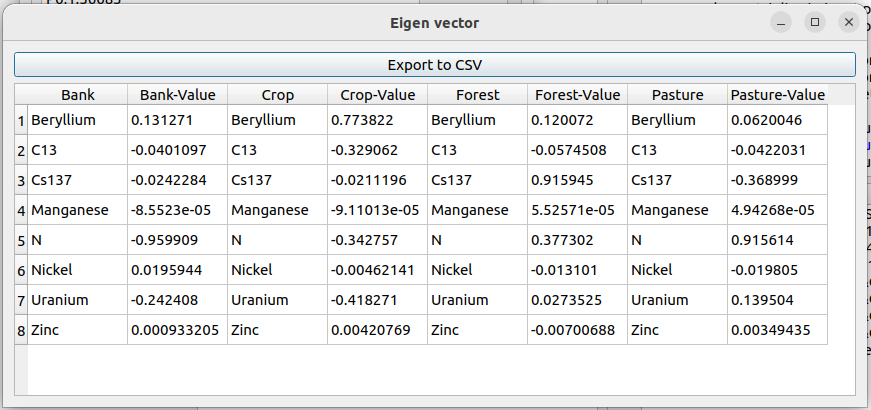
\includegraphics[width=14cm]{Figures/Multiway-DFA-eigenvectors.png}
    \caption{Estimated eigenvectors based on maximizing the separation of samples in each source with all other samples.}
    \label{fig:Multiway-eigenvectors}
\end{figure}
\FloatBarrier


\section{Fingerprinting}
The Levenberge-Marquardt Maximum likelihood estimation (LMMLE) is the simplest method implemented in SedSAT3. LMMLE uses the Levenberge-Marquardt optimization method to maximize the log-likelihood in Eq. \eqref{eq:loglikelihood-eqstd}. The transformation function $g$ is assumed to be log-normal, and the scale factor $\sigma$ of the log-normal distribution is assumed to be the same for all the elements. 

Modeled target sample elemental profile, $\mathbf{C}$ is calculated based on the arithmetic average of the elemental profiles of all samples in each source group (i.e., Eq. \eqref{eq:y_avg}). 

To perform LMMLE from the tools window, select \textbf{Tools}$\rightarrow$\textbf{Fingerprinting tools}$\rightarrow$\textbf{Levenberg-Marquardt optimization}. 

Checking the "Apply size and organic correction" will perform size and organic correction on the source samples if size and organic correction is done previously. It will use the latest size and correction model selected. The size and correction will be applied to the elements, size, and/or organic matter based on what is indicated in \textbf{Settings}$\rightarrow$\textbf{Organic matter/Size correction}. 

If no organic matter/size correction has been performed on the data, an error message will be shown asking it to be performed. You have the option to check off the OM and size correction and proceed or to perform OM and size correction. 

Choose the target sample you would like to be analyzed using the drop-down menu labeled Target Sample. The soft-max transformation maps the elemental contributions from $[0,1]$ domain to $[-\infty, \infty]$ domain through the Softmax transformation: 

\begin{equation}
    x_i = \frac{e^{\zeta_i}}{\sum_{i=1}^n e^{\zeta_i}}
\end{equation}

And the optimization is done for $\zeta$ values rather than $x$ values. Using the Softmax transformation implicitly imposes the constraint of the summation of contributions being 1.0 (Eq. \eqref{eq:sum}), and the search in the infinite domain is more efficient than the search in $[0,1]$ domain. 

Click the Ok button at the bottom of the form. The progress window will show the Mean Squared Error (MSE) value as the Levenberge-Marquardt iterations proceed. After the iterations converge, the result window will appear. The result window contains four panels. The first panel contains the inferred contributions of the source groups. You can click on the graph button 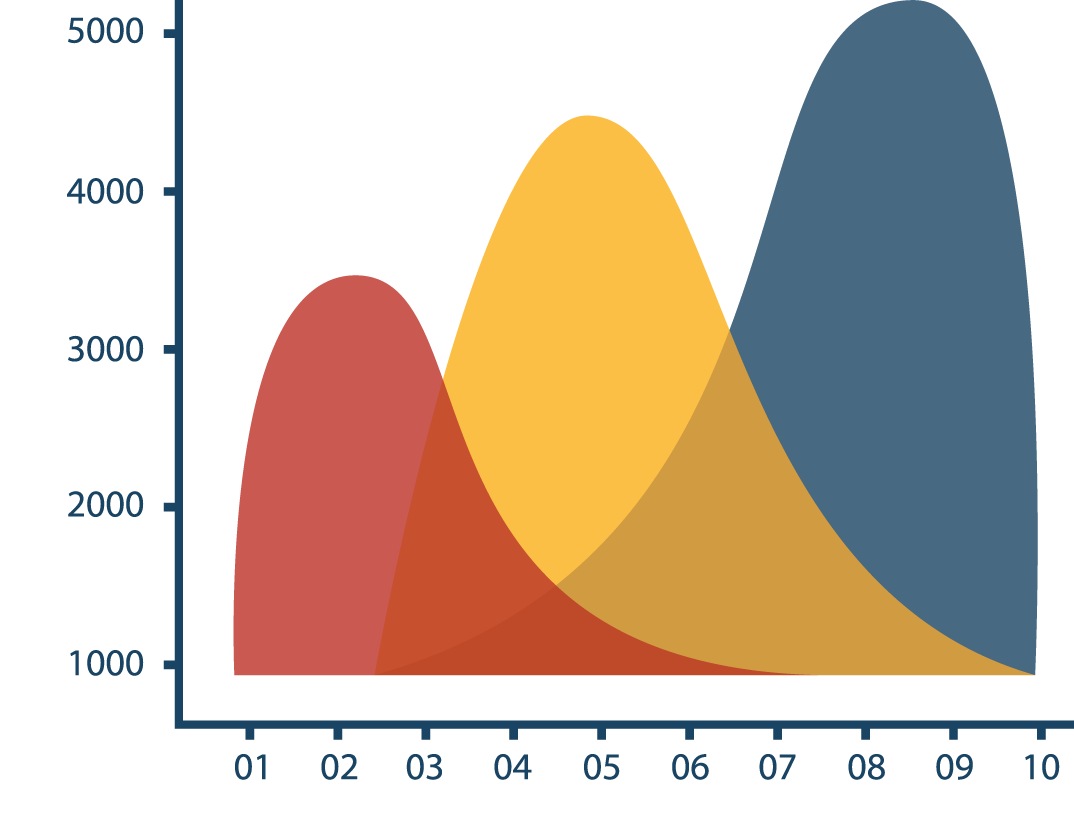
\includegraphics[width=0.5cm]{Figures/Graph.png} on the side of the panel to see the results as a pie chart (Figure \ref{fig:contribution_pie_chart}). 

\begin{figure}[ht]
    \centering
    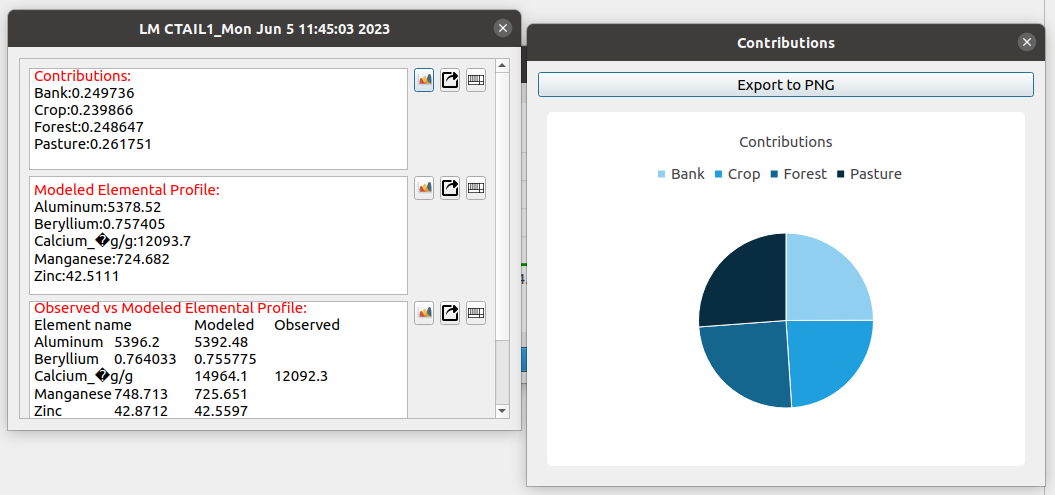
\includegraphics[width=15cm]{Figures/Contribution_Pie_Chart.png}
    \caption{Source contributions obtained from the LMMLE method}
    \label{fig:contribution_pie_chart}
\end{figure}
\FloatBarrier

The second panel shows the modeled target sample elemental profiles, $\mathbf{C}$. The third panel contains modeled and observed elemental profiles. We can use this to evaluate how close the elemental profile as a result of the mixing of the source groups is to the observed sample's elemental profile. Click on the graph button 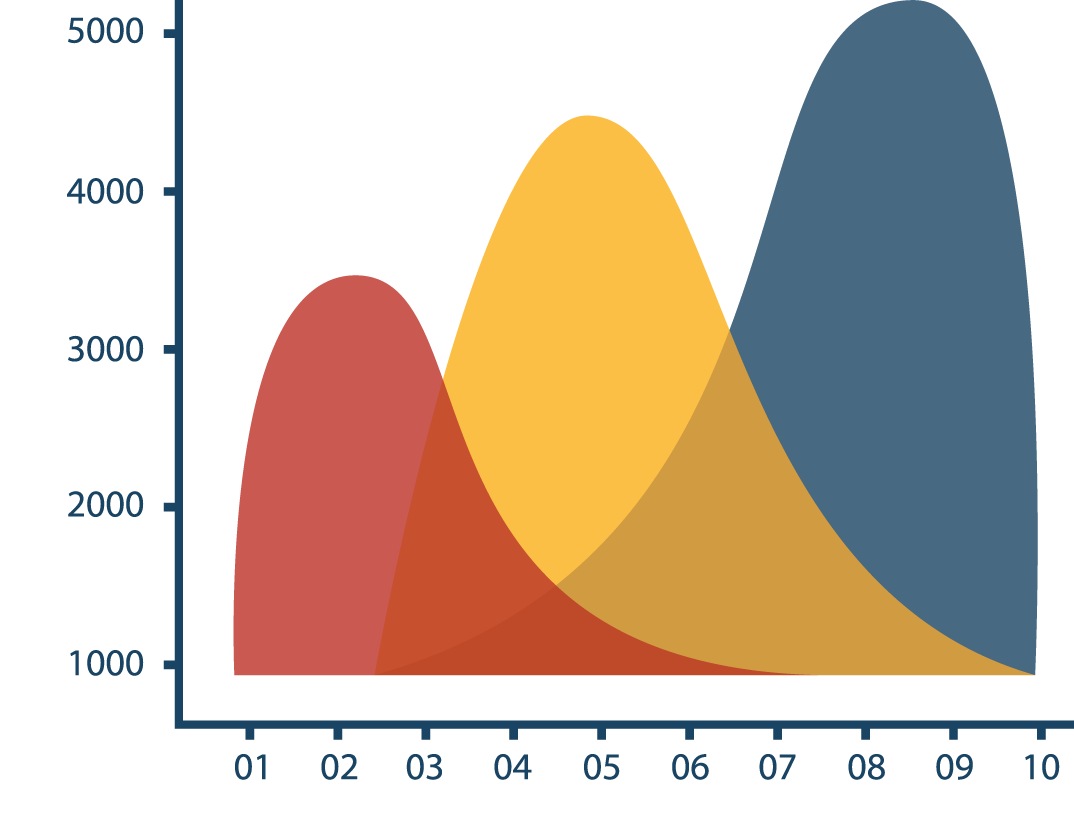
\includegraphics[width=0.5cm]{Figures/Graph.png} on the side of the panel to see the matching between modeled and observed elemental profiles graphically (Figure \ref{fig:LMMLE_modeled_vs_measured}).  

\begin{figure}[ht]
    \centering
    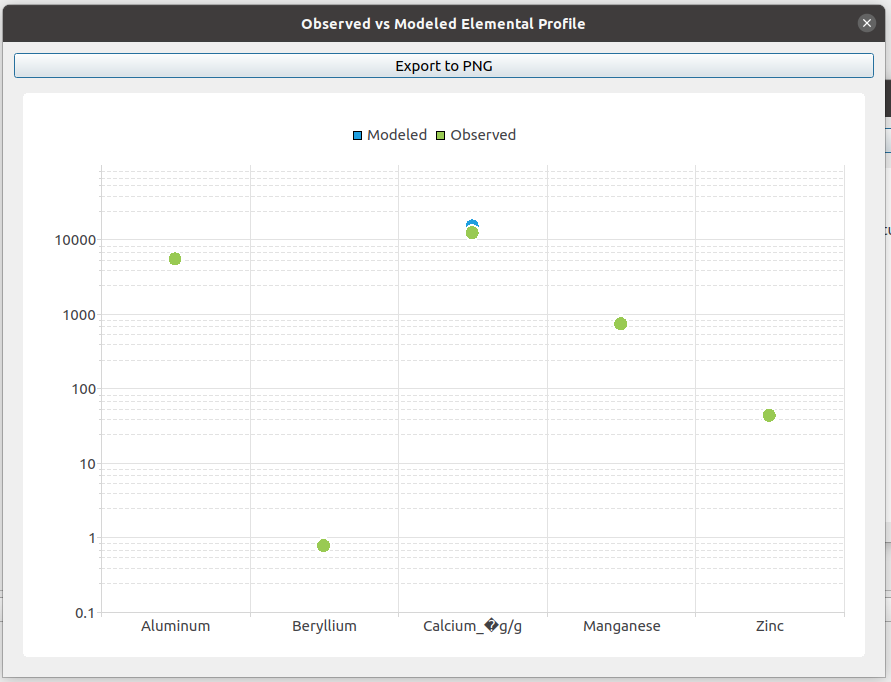
\includegraphics[width=10cm]{Figures/LMMSE_modeled_vs_measured.png}
    \caption{Modeled vs. observed Elemental profiles }
    \label{fig:LMMLE_modeled_vs_measured}
\end{figure}
\FloatBarrier

And finally, the fourth panel contains the modeled vs. measured results for the isotope ratios in case constituents contain some isotopes. 


\section{Fingerprinting (Batch)}

This tool performs the Levemberge-Marquardt maximum likelihood fingerprinting for all target samples simultaneously. To perform batch Levenberge-Marquardt fingerprinting, select \textbf{Tools}$\rightarrow$\textbf{Fingerprinting tools}$\rightarrow$\textbf{Levenberg-Marquardt optimization (Batch)}. Select whether you want the OM and size correction to be applied to the source samples and whether the soft-max transformation is to be used. Click on the "OK" button.  Wait until the process is completed. The batch version of the LM fingerprinting provides fewer details than when performing the analysis on each target sample individually. The resulting panel only shows the estimated source contribution for each target sample. Click on the graph button 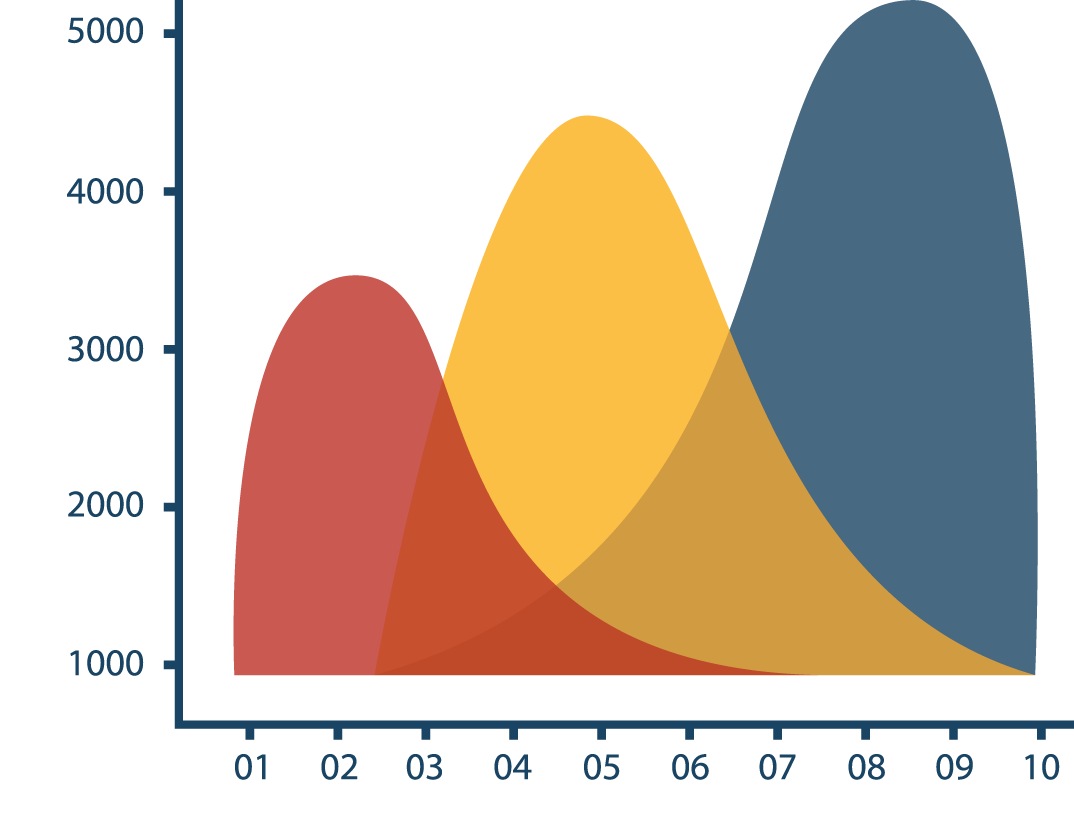
\includegraphics[width=0.5cm]{Figures/Graph.png} to see the contribution of each source to each target sample graphically (Fig. \ref{fig:LM-Batch-results-graph}) and the table button to see the results in a tabular form (Fig. \ref{fig:LM-Batch-results-table}). 

\begin{figure}[ht]
    \centering
    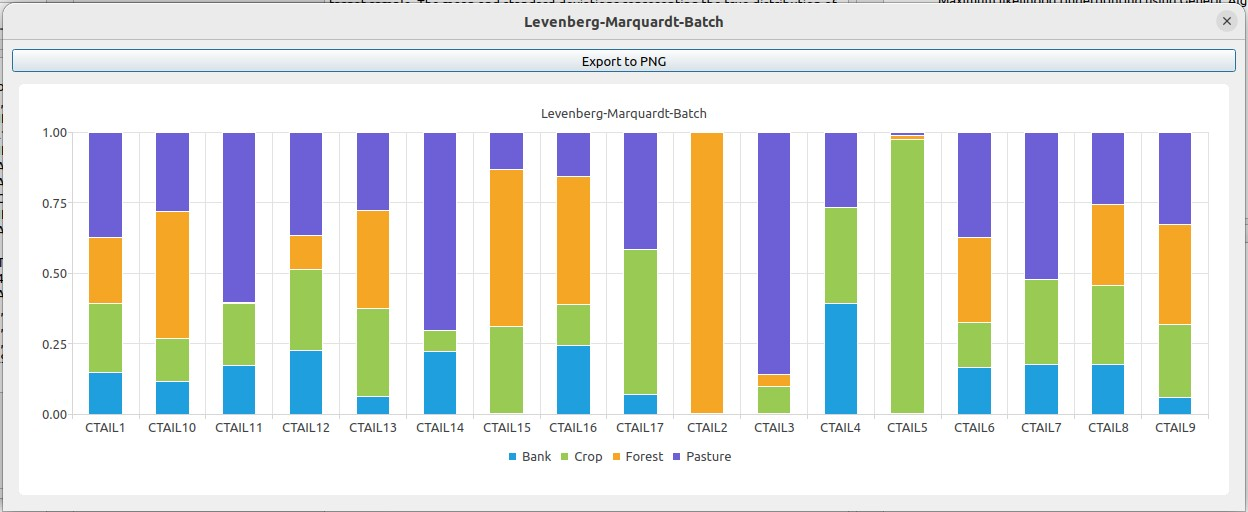
\includegraphics[width=14cm]{Figures/LL-batch-graph.png}
    \caption{The graph showing the Levenberg-Marquardt batch results}
    \label{fig:LM-Batch-results-graph}
\end{figure}
\FloatBarrier

\begin{figure}[ht]
    \centering
    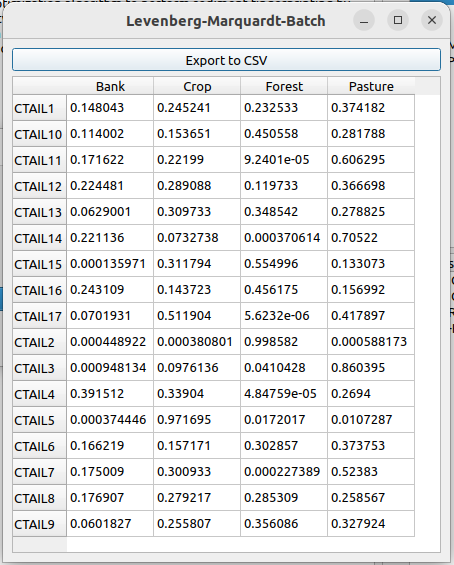
\includegraphics[width=8cm]{Figures/LL-batch-table.png}
    \caption{Levenberg-Marquardt batch results in tabular format}
    \label{fig:LM-Batch-results-table}
\end{figure}
\FloatBarrier



\chapter{Bayesian Sediment Fingerprinting}
This chapter covers the Bayesian fingerprinting method implemented in \textit{SedSat}. The pre-analysis steps required for Bayesian fingerprinting—namely, \textit{Outlier Analysis}, \textit{Organic Matter and Particle Size Correction}, \textit{Bracketing Analysis}, and \textit{Stepwise Discriminant Function Analysis}—were presented in the previous chapter. The focus here is on the Bayesian sediment fingerprinting procedure, which produces the final results of the analysis.

\section{Bayesian Chemical Mass Balance Analysis}
As it was mentioned in section \ref{sec:basic_concepts_bayesian}, there are various sources of uncertainty in sediment fingerprinting. These include but are not limited to measurement errors, lack of representativeness of source samples, presence of unidentified sources, or equifinality. The Bayesian approach provides a probability distribution for the source contributions rather than providing point estimates based on the maximum likelihood estimation. 

To perform Bayesian fingerprinting from the tools window, select \textbf{Tools}$\rightarrow$\textbf{Bayesian Sediment Finger Printing}$\rightarrow$\textbf{Bayesian Chemical Mass Balance Analysis}. 

Below are the descriptions of the setting items appearing in the central form:

\begin{itemize}
    \item \textbf{Apply size and organic matter correction: } indicates whether the analysis is performed on the corrected elemental profiles based on size and organic matter. Note that in order to size and organic correction to be done, a size and organic matter correction step (section \ref{sec:sizeandorganiccorrection}) should have been performed before. 
    \item \textbf{Dissolve Chains: } This option indicates that during the Markov chain Monte Carlo (MCMC) sampling, chains with significantly lower posterior probability will be discarded and replaced by chains with higher posterior probability. This will improve the convergence speed of the algorithm. 
    \item \textbf{Number of Chains: } The number of MCMC chains to be used in parallel. 
    \item \textbf{Number of Samples: } Indicates the total number of samples to be generated. For a full convergence, typically, 100,000 samples or more are necessary. 
    \item \textbf{Sample: } The label of the target sample to be analyzed. 
    \item \textbf{Samples file name: } Indicate the text file where MCMCM samples information will be saved in. 
    \item \textbf{Samples to be discarded (burnout): } Indicate the number of samples to be discarded from the beginning of MCMC chains. If the total number of samples is 100000, it is recommended that the burnout be specified as 20000. 
\end{itemize}

After setting the parameters, click on the Ok button to start the analysis. The analysis duration depends on the number of samples indicated to be produced. 

The progress window contains some information that can shed light on suitable parameters for MCMC sampling. 

\begin{figure}[ht]
    \centering
    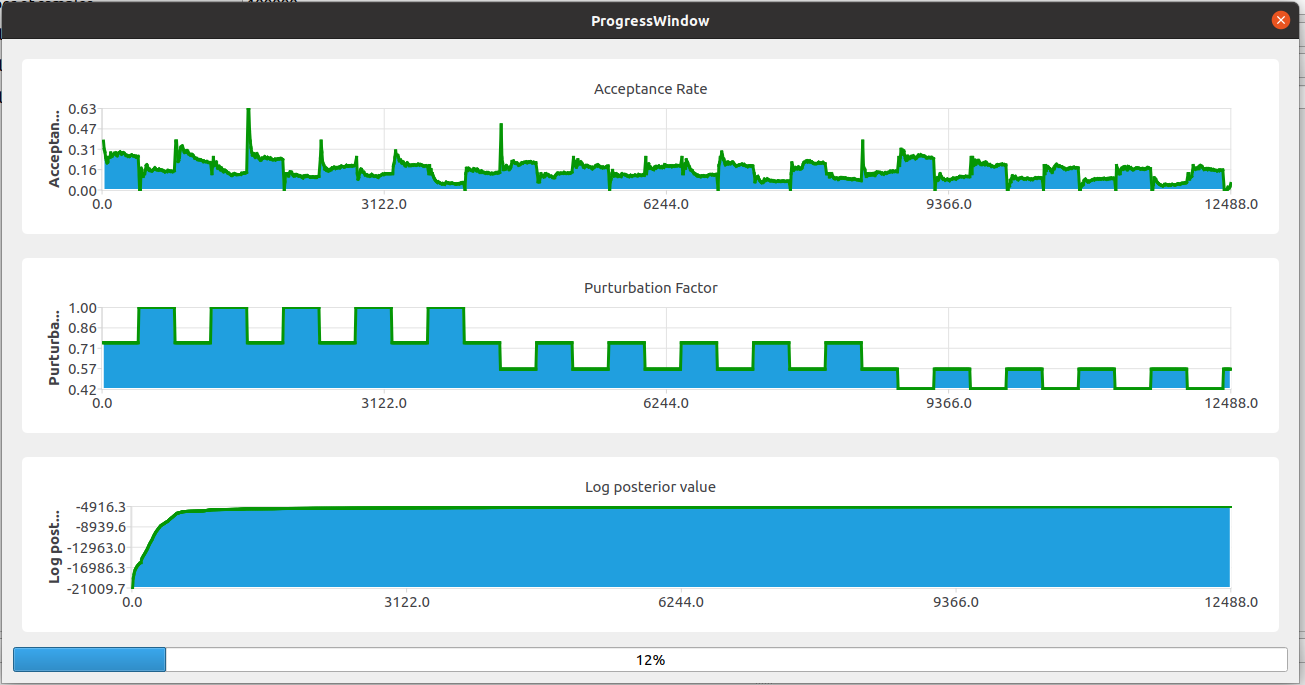
\includegraphics[width=14cm]{Figures/MCMC_progress.png}
    \caption{Progress window of Bayesian chemical mass balance analysis}
    \label{fig:MCMC-progress}
\end{figure}
\FloatBarrier

The top panel shows the average acceptance rate (i.e., the fraction of accepted new samples). The perturbation factor (panel 2) is adjusted to maintain an acceptance rate of around 15\%. The bottom panel shows the maximum numerator of the posterior distribution (Eq. \eqref{eq:Bayesian-Prop}). Initially, the values are lower when the samples are far from the maximum likelihood estimates. As the algorithm proceeds, the values increase and eventually are stabilized. The number of discarded samples can be indicated based on the number of samples that it will take for the value shown on this chart to stabilize. 

After the MCMC sampling is finished, a result window will pop up. The result window contains five panels. 

The first panel contains MCMC samples for each parameter, including source contributions, $\mu$, and $\sigma$ values of log-normal distributions considered for the elemental content of each source group and the error standard deviations (Figure \ref{fig:MCMC-samples}). Click on the graph button 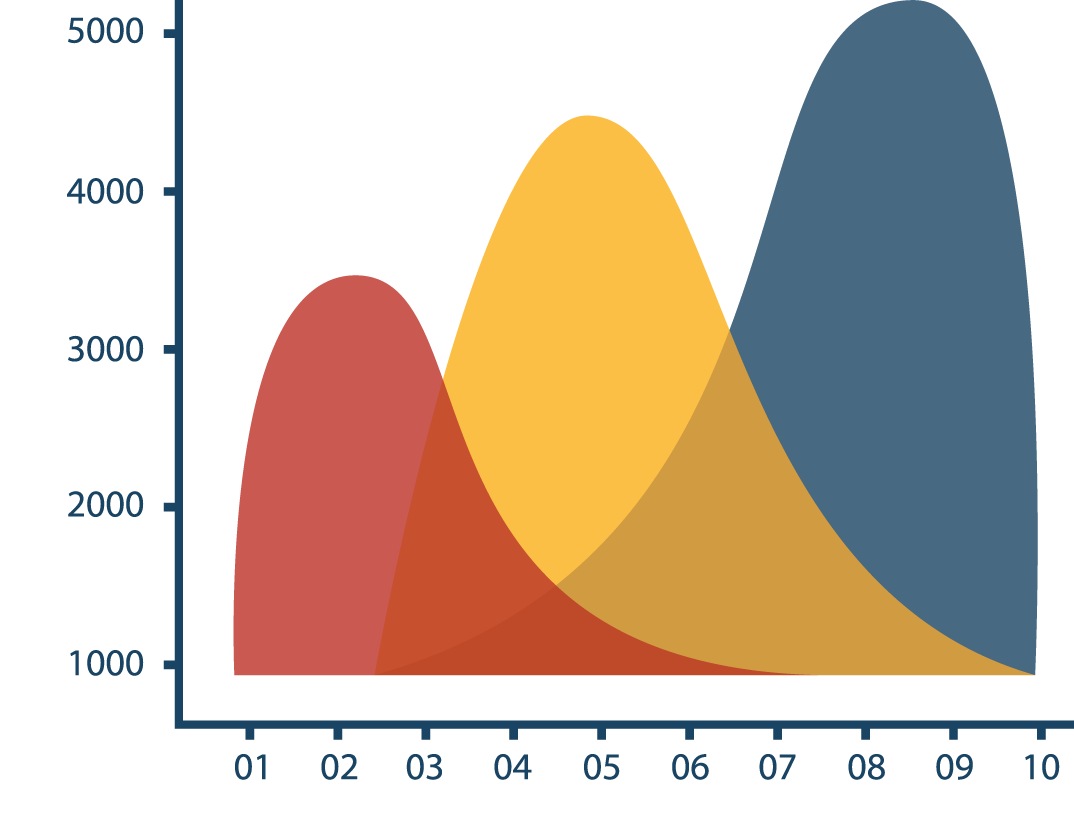
\includegraphics[width=0.5cm]{Figures/Graph.png} to see the visualization of the samples (Figure \ref{fig:MCMC-samples}). Use the drop-down menu at the top to see the results for different parameters. Note the convergence of the results. For example, based on figure \ref{fig:MCMC-samples}, it seems that the algorithm takes around 25000 samples to converge as indicated by the bank and crop contribution parameter. 

\begin{figure}[ht]
    \centering
    \begin{tabular}{c c}
        a) & b) \\
        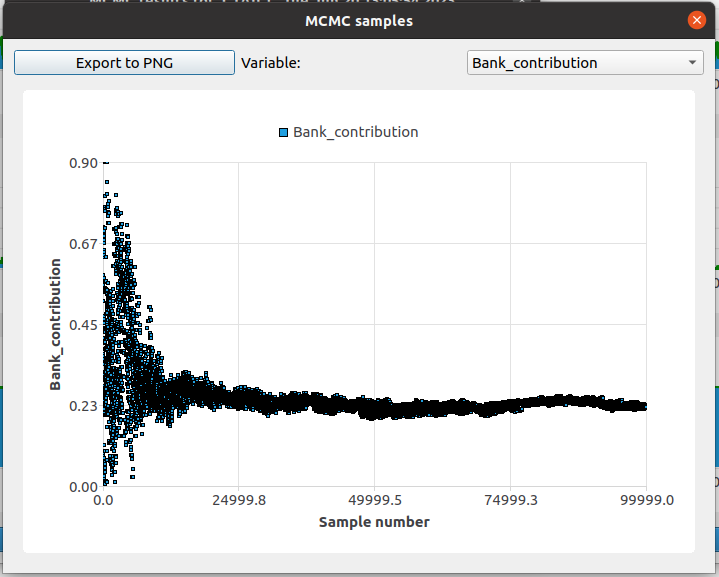
\includegraphics[width=8cm]{Figures/MCMC_Samples_Bank.png} & 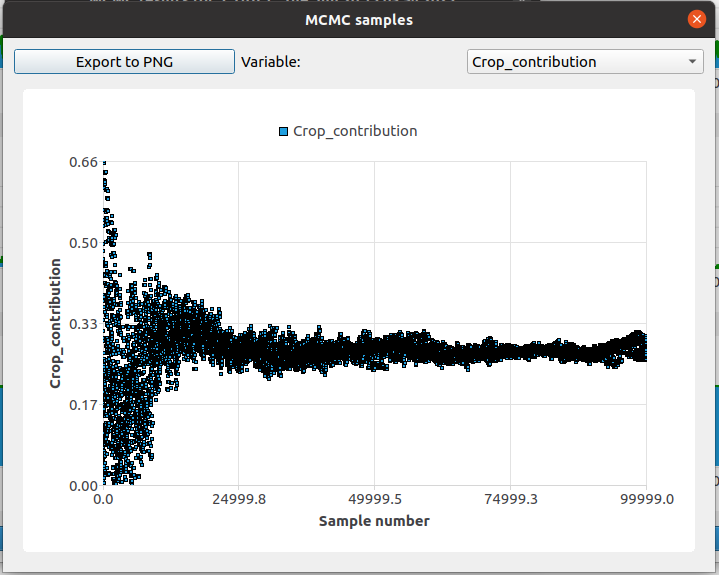
\includegraphics[width=8cm]{Figures/MCMC_samples_crop.png}
    \end{tabular}
    \caption{Visualization of MCMC samples a) bank contribution samples. b) crop contribution samples}
    \label{fig:MCMC-samples}
\end{figure}
\FloatBarrier

Panel two can be used to visualize the posterior distribution based on the samples drawn. Click on the graph button 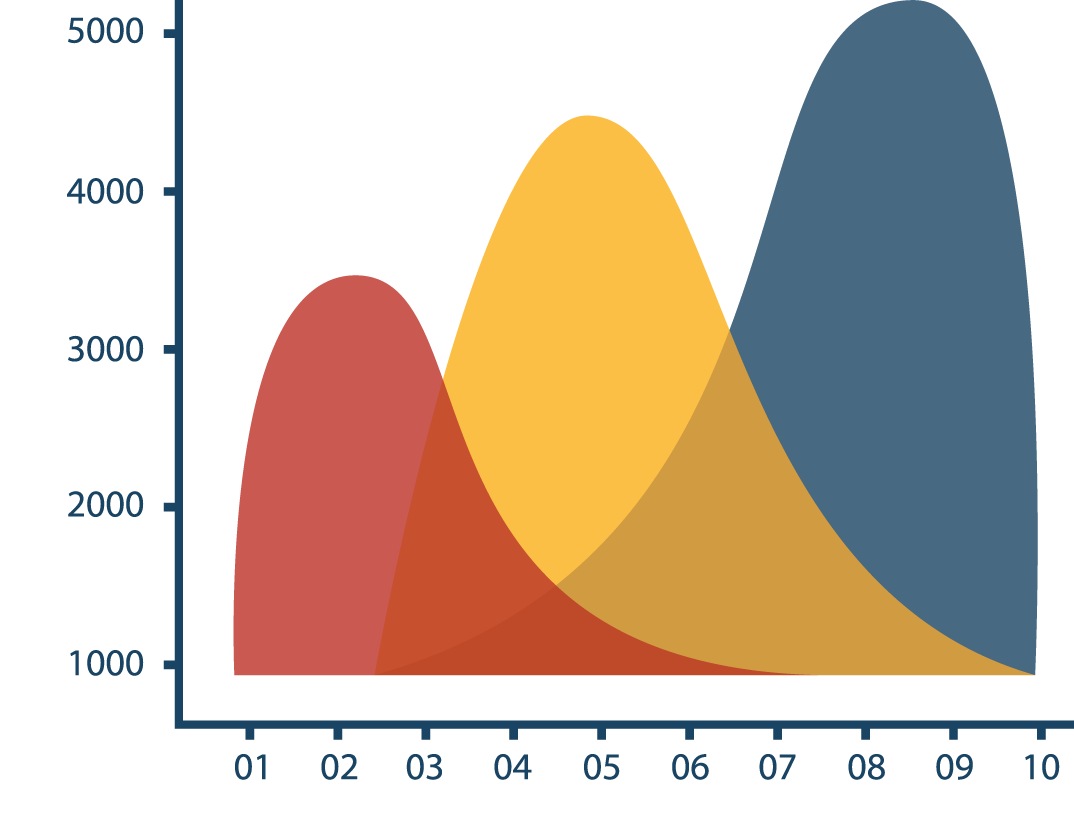
\includegraphics[width=0.5cm]{Figures/Graph.png} to see the posterior distributions for all the parameters. 

\begin{figure}[ht]
    \centering
    \begin{tabular}{c c}
        a) & b) \\
        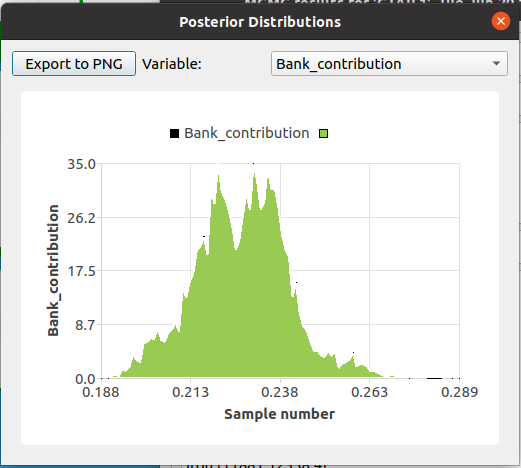
\includegraphics[width=8cm]{Figures/MCMC_Bank_Distribution.png} & 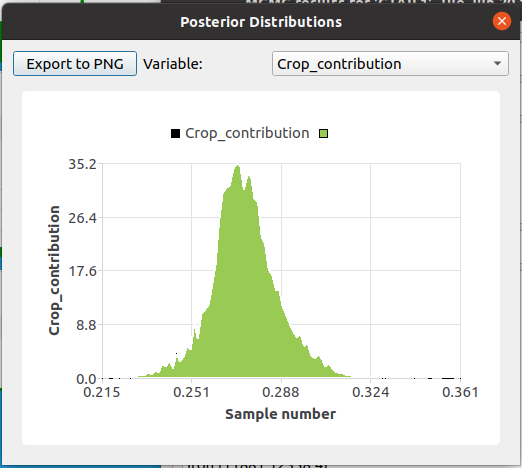
\includegraphics[width=8cm]{Figures/MCMC_crop_distribution.png}
    \end{tabular}
    \caption{Visualization of the posterior distribution for a) bank contribution and b) crop contribution}
    \label{fig:MCMC-distributions}
\end{figure}
\FloatBarrier

The third panel contains the 95\% credible intervals of source contributions. The credible interval is the range the source contribution falls in with 95\% probability (Figure \ref{fig:MCMC-credible-interval}). In addition to the low and high ranges of the credible intervals, the table also shows the expected value (mean) and median from the posterior distributions. 

Click on the table button 
\includegraphics[width=0.5 cm]{Figures/table.png} on the side of the panel to see the range in tabular form. Click on the graph button 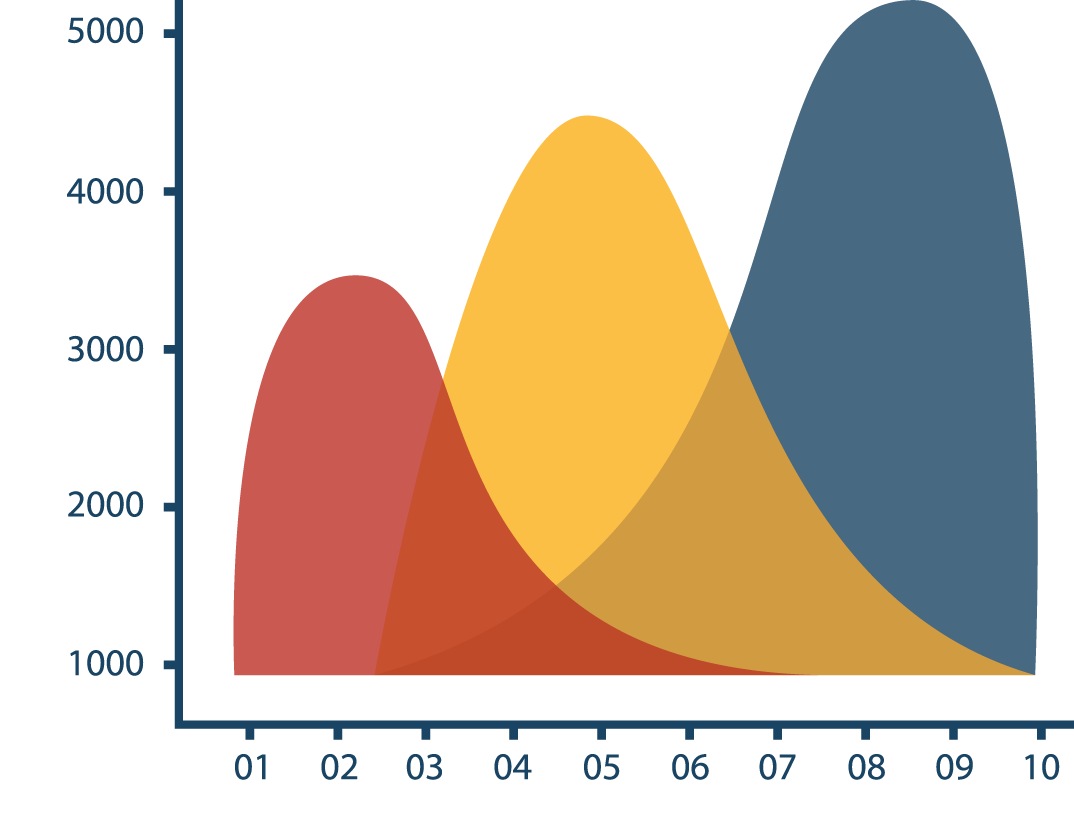
\includegraphics[width=0.5 cm]{Figures/Graph.png} to see the credible intervals graphically. 

\begin{figure}[ht]
    \centering
    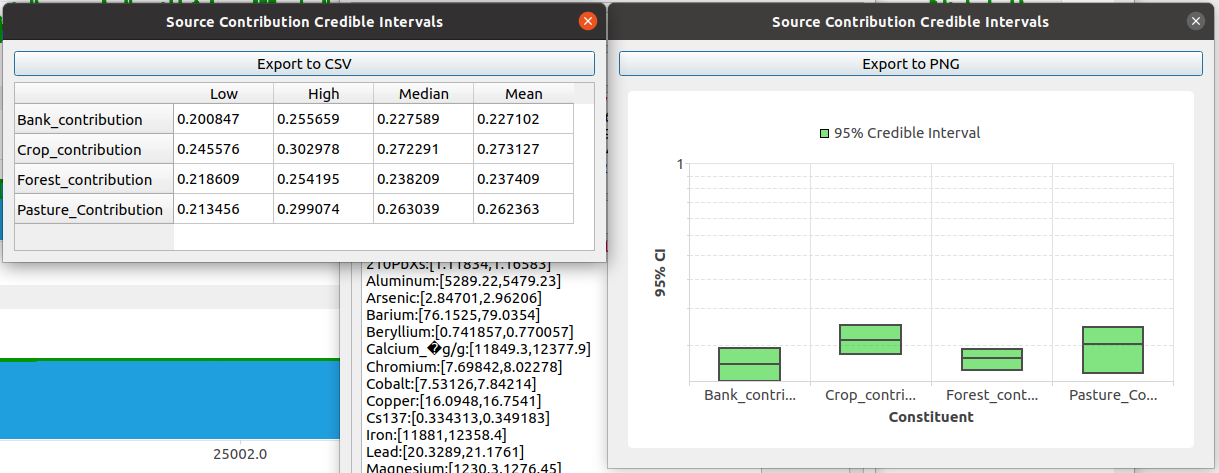
\includegraphics[width=14cm]{Figures/MCMC-credible-intervals.png} 
    \caption{Credible intervals for source contributions}
    \label{fig:MCMC-credible-interval}
\end{figure}
\FloatBarrier

The fourth panel in the Bayesian analysis result window contains the predicted (posterior) distribution of element contents in the target sample. Click on the graph button 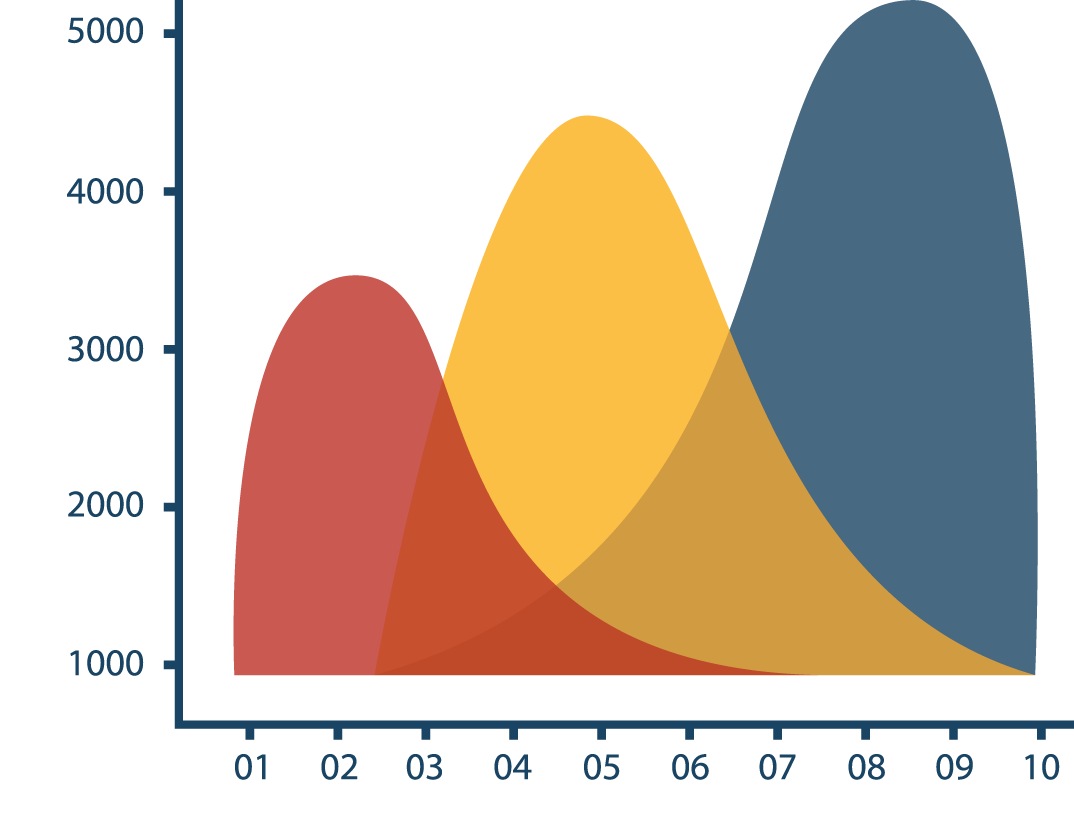
\includegraphics[width=0.5 cm]{Figures/Graph.png} to see the distributions graphically. Use the drop-down menu at the top of the graph to see the predicted distribution for each element (Figure \ref{fig:MCMC-posterior-elemental-content}). The distribution is obtained by calculating the target elemental profile for each MCMC sample. The vertical dashed line in the graph shows the measured concentration in the target sample. 

\begin{figure}[ht]
    \centering
    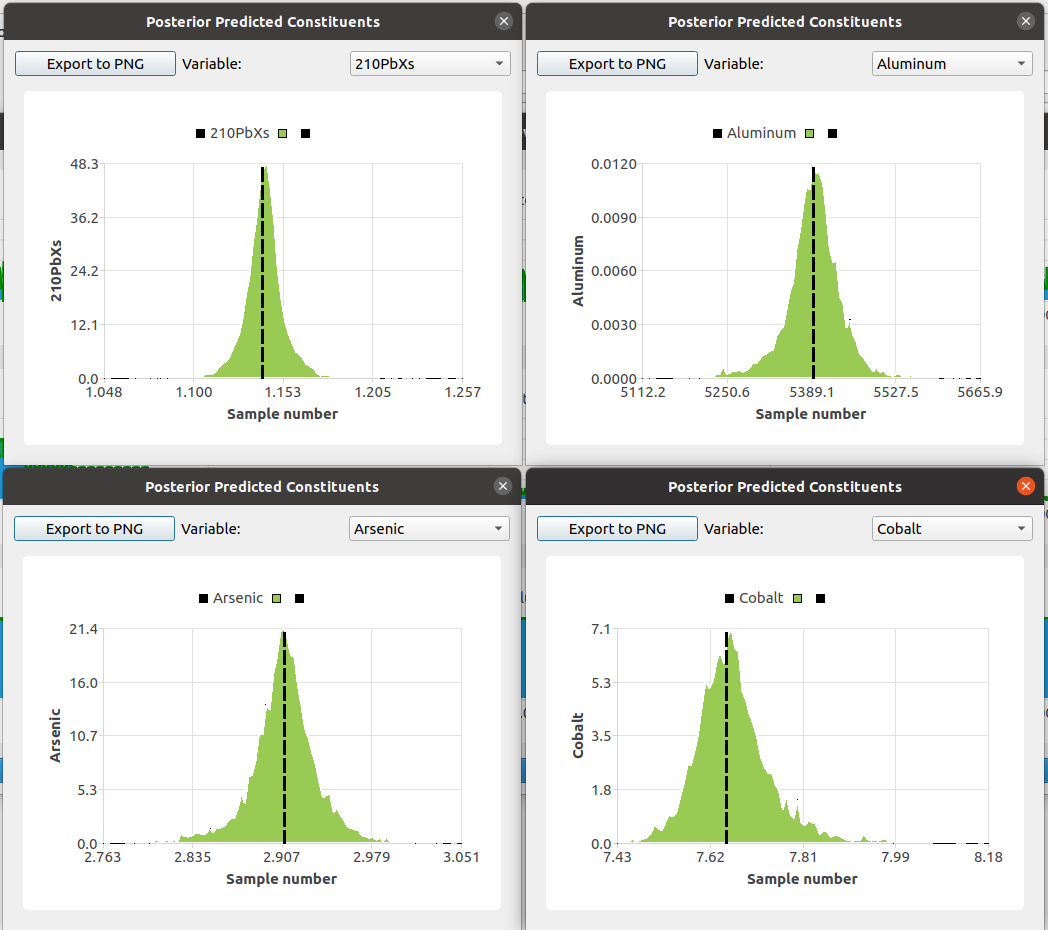
\includegraphics[width=14cm]{Figures/MCMC_Posterior_Elemental_Contents.png} 
    \caption{Posterior distribution of elemental contents in the target sample}
    \label{fig:MCMC-posterior-elemental-content}
\end{figure}
\FloatBarrier

The 95\% credible intervals of predicted elemental contents in the target sample can be found in panel five of the result window. Click on the table button 
\includegraphics[width=0.5 cm]{Figures/table.png} on the side of the panel to see the range in tabular form. Click on the graph button 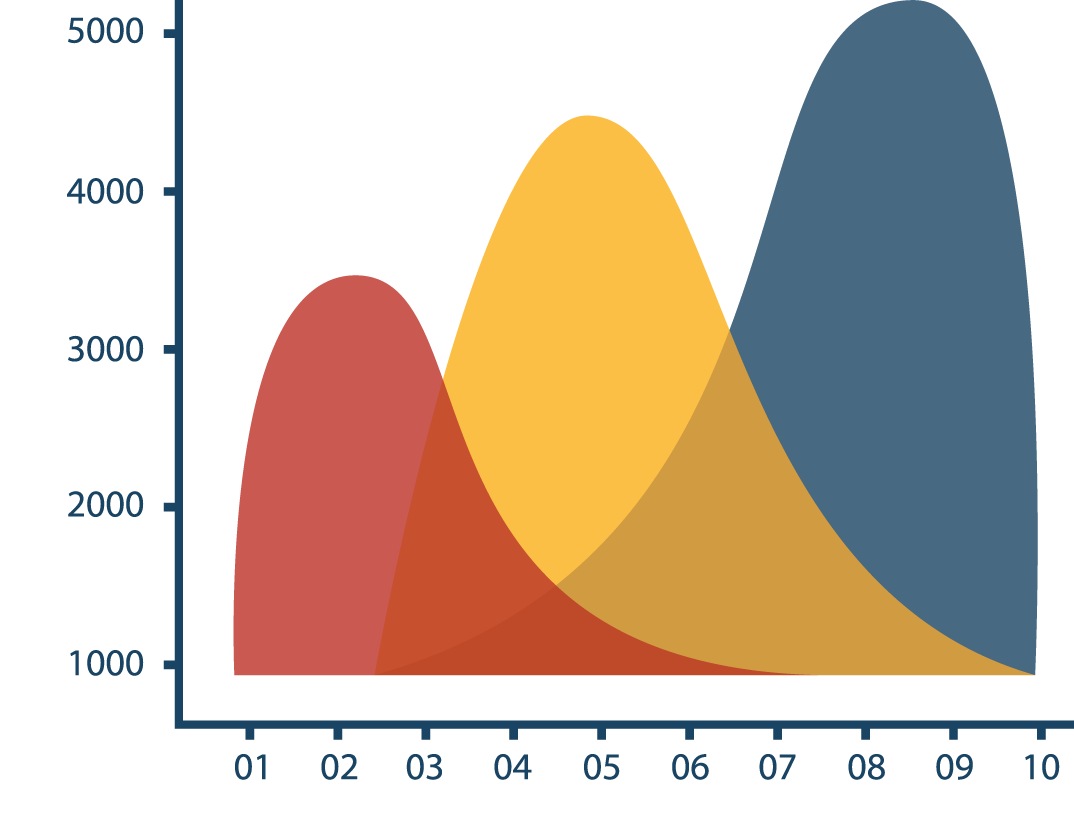
\includegraphics[width=0.5 cm]{Figures/Graph.png} to see the credible intervals graphically. The graph will also include the measured elemental content in the target sample for each element with dot symbols. The difference between the 95\% bracket and the measured value will give us an insight into how well each elemental content can be captured based on the combination of the sources.

Panels six and seven contain similar information to panels four and five but for isotopes if isotopes are included in the analysis. 

\section{Bayesian Chemical Mass Balance Analysis (Batch)}
The batch version of the Bayesian Chemical Mass Balance tool conducts Bayesian fingerprinting on all target samples, saving users from selecting samples one by one and manually saving the analysis. Instead of displaying detailed results as tables and graphs, the analysis outputs are saved in text files that can be easily plotted using standard spreadsheet programs or graphing software applications. The settings are the same as described for the Bayesian Chemical Mass analysis tool. 

To perform batch Bayesian chemical mass balance analysis, from the tools window, select \textbf{Tools}$\rightarrow$\textbf{Bayesian Sediment Fingerprinting}$\rightarrow$\textbf{Bayesian Chemical Mass Balance Analysis (Batch)}. 

Note that a large number of samples (>100,000) is required for the results to converge, and approximately 10\% of the total samples should be designated as burn-in. The analysis can take considerable time, depending on the number of target samples, source groups, and MCMC samples, as well as your hardware's processing power.

After the analysis is complete, folders named after your target samples will be created in the same directory where the project is saved (Figure \ref{fig:MCMC-folders}). Each folder will contain seven text files (Figure \ref{fig:MCMC-files}).

\begin{figure}[ht]
    \centering
    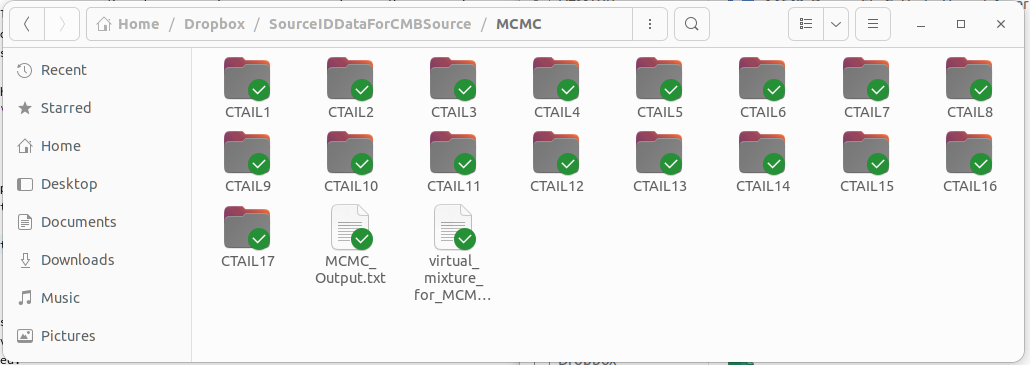
\includegraphics[width=14cm]{Figures/MCMC_folders.png} 
    \caption{The folders created after performing batch Bayesian chemical mass balance modeling}
    \label{fig:MCMC-folders}
\end{figure}
\FloatBarrier

\begin{figure}[ht]
    \centering
    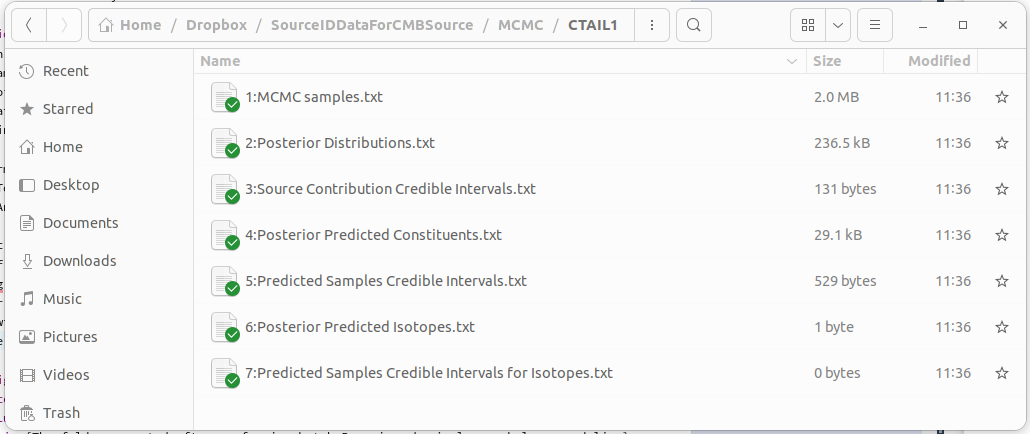
\includegraphics[width=14cm]{Figures/MCMC_files.png} 
    \caption{Text files containing the batch Bayesian chemical mass balance modeling results}
    \label{fig:MCMC-files}
\end{figure}
\FloatBarrier

The files include: 

\begin{itemize}
    \item \textbf{1:MCMC samples.txt}: This file contains all the MCMC samples generated. The columns represent the estimated parameters, including the source contribution values for each source, the mean and standard deviation of each element in each source group, and the likelihood values for each parameter set.
    \item \textbf{2:Posterior Distributions.txt}: This file contains the MCMC samples converted into frequency distributions. The columns come in pairs, the first one containing the values of the parameters and the second containing the value of the frequency distributions. For example, in order to plot the posterior distribution of "Bank Contribution", column B should be plotted vs. column A and so forth. 
    \item \textbf{3:Source Contribution Credible Intervals.txt}: This file contains the 95\% credible intervals of each parameter extracted from the posterior distribution (Figure \ref{fig:posterior-95-table}).

    \begin{figure}[ht]
    \centering
    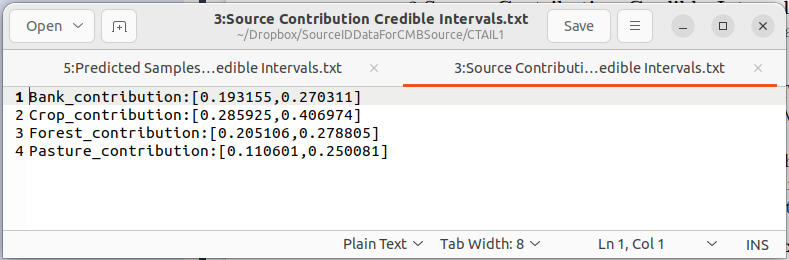
\includegraphics[width=14cm]{Figures/95p_CI_table.png} 
    \caption{Text files containing 95\% credible intervals of model parameters}
    \label{fig:posterior-95-table}
    \end{figure}
    \FloatBarrier
    
    \item \textbf{4:Posterior Predicted Constituents.txt}: This file contains predicted target sample concentrations based on the drawn MCMC samples converted into frequency distributions. The columns come in pairs, the first one containing the values of predicted elemental content and the second containing the value of the frequency distributions. For example, in order to plot the frequency distribution of $^{210}Pb$, column B should be plotted against column A. 
    
    \item \textbf{5:Predicted Samples Credible Intervals.txt}: This file contains the 95\% credible intervals of the predicted target sample elemental profile based on the parameters extracted from Posterior Predicted Constituents (Figure \ref{fig:posterior-95-predicted-table}).

    \begin{figure}[ht]
    \centering
    \includegraphics[width=14cm]{Figures/95p_CI_predicted.png} 
    \caption{Text files containing 95\% credible intervals of predicted target sample elemental content}
    \label{fig:posterior-95-predicted-table}
    \end{figure}
    \FloatBarrier
    
    \item \textbf{6:Posterior Predicted Isotopes.txt}: This file contains predicted target isotope ratios based on the drawn MCMC samples converted into frequency distributions. The columns come in pairs, the first one containing the values of predicted isotope ratios and the second containing the value of the frequency distributions. This file will be empty if your analysis contains no isotopes.
    \item \textbf{7:Predicted Samples Credible Intervals for Isotopes.txt}: This file contains the 95\% credible intervals of the predicted target sample isotope ratios based on the parameters extracted from Posterior Predicted Isotopes.
\end{itemize}

\chapter{Other Statistical Tools}
The miscellaneous analysis tools provide some non-essential statistical tools for analyzing fingerprinting data. Below, each tool is described.

\section{Elements' correlation matrix}
Knowing the correlation between constituents used for fingerprinting within source groups is useful information in deciding which constituents are to be used in the fingerprinting analysis. 

The value of the correlation between each two elements $j$ and $j'$ in a source group $i$ is calculated as: 


\begin{equation}
    r_{j,j'} = \frac{\sum\limits_{k}^{} (y_{j,k}-\bar{y}_j)(y_{j',k}-\bar{y}_{j'})}{\sqrt{\sum\limits_{k}^{}(y_{j,k}-\bar{y}_j)^2\sum\limits_{k}^{}(y_{j',k}-\bar{y}_{j'})^2}}
\end{equation}

where $y_{j,k}$ and $y_{j',k}$ are respectively the measured elemental contents of elements $j$ and $j'$ in sample $k$ in the source group, and $\bar{y}_j$ and $\bar{y}_{j'}$ are the average elemental contents of elements $j$ and $j'$ respectively in the source group. 

From the "Tools" menu in the far right window panel, double-click on \textbf{Pre-Analysis tools}$\rightarrow$\textbf{Elements' correlation matrix}. Choose the source/target group for which you want the correlation matrix calculated from the drop-down menu labeled Source/Target group. The text box labeled threshold indicates the threshold above which the values will be highlighted. If you check the \textit{Use only selected elements} item, the correlation matrix will be generated only for the elements indicated to be included in the analysis in \textbf{Settings}$\rightarrow$\textbf{Constituent properties}. Also, checking the \textit{Use only selected samples} checkbox only includes the samples that are indicated to be included in the analysis in \textbf{Settings}$\rightarrow$\textbf{Include/Exclude samples}. Click the Ok button at the bottom of the form, and a window, like in Figure \ref{fig:correlation_matrix}, will appear. Click on \includegraphics[width=0.5 cm]{Figures/table.png} button to see the matrix in a tabular form (Fig. \ref{fig:correlation_table}). You can export the results to a .csv file by clicking on \includegraphics[width=0.5 cm]{Figures/export.png}. At this point, based on the correlation matrix, the user can make a decision on which tracers to remove from further analysis.  To remove a tracer go to settings in the upper left hand corner of the screen, click on  Constituent Properties and  double click on "include in analysis" the element you want to remove. To conduct the correlation analysis on the source elemental profiles adjusted for size, organic matter, or both, select the target sample on which you would like the correction to be based.  Under the results window panel located beneath the Tools panel, your results will be stored for you. You can go back and re-review any. 

\begin{figure}[ht]
    \centering
    \includegraphics[width=10cm]{Figures/Correlation_Matrix.png}
    \caption{Correlation matrix results}
    \label{fig:correlation_matrix}
\end{figure}


\begin{figure}[ht]
    \centering
    \includegraphics[width=10cm]{Figures/Correlation_Table.png}
    \caption{Correlation matrix table}
    \label{fig:correlation_table}
\end{figure}

\FloatBarrier

Based on the correlation analysis results, the user can decide if a tracer should be eliminated from further analysis. Usually, this decision is made for a tracer that has a high correlation to the same tracer(s) for all source groups. Once a decision is made the user should go to the Setting tab and under constituent properties remove that tracer.

\section{Analysis of Variance}
Analysis of Variance (ANOVA) facilitates the evaluation of the effectiveness of different elements in distinguishing between source groups by comparing the variations in elemental content both between and within these groups. This analysis aids in identifying elements that possess a greater capacity for fingerprinting by highlighting those with significant differences in their distribution across the groups.

The one-way ANOVA (Analysis of Variance) is a statistical technique used to compare means of three or more samples (assuming equal variances) to determine if at least one sample mean is significantly different from the others. It does this by analyzing the variance within each group and the variance between the groups. The formula for one-way ANOVA involves calculating the F-statistic, which is the ratio of the variance between the groups to the variance within the groups. The formula for the F-statistic in one-way ANOVA is:

\begin{equation}
    F = \frac{MS_{between}}{MS_{within}}    
\end{equation}

where:

$F$ is the F-statistic, $MS_{between}$ (Mean Square Between) is the variance between the groups, and $MS_{within}$ (Mean Square Within) is the variance within the groups.

The Mean Square Between ($MS_{between}$) is calculated as:

\begin{equation}
    MS_{between} = \frac{SS_{between}}{df_{between}}    
\end{equation}

And the Mean Square Within ($MS_{within}$) is calculated as:

\begin{equation}
    MS_{within} = \frac{SS_{within}}{df_{within}}    
\end{equation}

where:

- $SS_{between}$ (Sum of Squares Between) is the sum of squares between the groups, \\
- $df_{between}$ (degrees of freedom between) is the number of groups minus one $(n - 1)$, \\
 - $SS_{within}$ (Sum of Squares Within) is the sum of squares within the groups, and \\
- $df_{within}$ (degrees of freedom within) is the total number of observations minus the number of groups $(l - n)$.

The Sum of Squares Between ($SS_{between}$) and Sum of Squares Within $SS_{within}$ are calculated using the following formulas:

\begin{equation}
    SS_{between} = \sum_{i=1}^{n} n_i (\bar{y}_i - \bar{y})^2    
\end{equation}

\begin{equation}
SS_{within} = \sum_{i=1}^{n} \sum_{j=1}^{n_i} (y_{ij} - \bar{y}_i)^2
\end{equation}

 

where:

- $n_i$ is the number of observations in group $i$, \\
- $\bar{y}_i$ is the mean of group $i$, \\
- $\bar{y}$ is the overall mean of all observations, \\
- $y_{i,k}$ is the $k^{th}$ observation in the $i^{th}$ group, and \\
- $n$ is the number of groups.

The result, $F$, is then used to calculate a p-Value for the element in question. 

\begin{equation}
    p = \Xi^{-1} (F, n-1, l)
\end{equation}

where $\Xi$ is the cumulative $F$ distribution with degrees of freedom of $n-1$ and $l = \sum_{i=1}^{n} n_i$ (the total number of samples in all groups). 

To perform analysis of variance in SedSat3, from the \textbf{Tools}$\rightarrow$\textbf{Pre-Analysis Tools}$\rightarrow$\textbf{Analysis of Variance}. You have the option to conduct the analysis using either log-transformed elemental contents, Box-Cox transformed elemental contents or their raw values. To conduct the correlation analysis on the source elemental profiles adjusted for size, organic matter, or both, select the target sample on which you would like the correction to be based. By selecting "Modify the included elements based on the results," elements that have p-values exceeding the specified "P-value threshold" will be automatically removed. This threshold is utilized to identify elements with a low capacity for discrimination. Upon finalizing your selections, click the "Ok" button to proceed. After the analysis is complete the result window will appear. 

Click on the graph button \includegraphics[width=0.5 cm]{Figures/Graph.png} to see the p-Values for each element graphically. You can also see the values in tabular form by clicking on the table \includegraphics[width=0.5 cm]{Figures/table.png} button. For example, Fig. \ref{fig:Anova_Results} shows that the discriminatory capability of Arsenic and Cobalt are low in the demonstration dataset.  

\begin{figure}[ht]
    \centering
    \includegraphics[width=14cm]{Figures/ANOVA_results.png} 
    \caption{Results of the ANOVA analysis}
    \label{fig:Anova_Results}
\end{figure}
\FloatBarrier

\section{Auto-select elements}
The auto-select tool identifies the minimum number of elements required to effectively distinguish between all pairs of source groups. It first performs a T-test for each combination of source groups, then selects a predetermined number of elements with the lowest p-values from each pair.

To use this tool select \textbf{Tools}$\rightarrow$\textbf{Pre-Analysis Tools}$\rightarrow$\textbf{Auto-select elements}. You may decide to include isotopes in the analysis and adjust the source elemental profiles based on size and organic matter. To apply the selection automatically, check the box labeled as "Modify the included elements based on the results". The value of "Number of elements from each pair" indicates the number of elements with the lowest p-value that will be selected from each pair of source groups. A larger number results in a larger total number of selected elements. Click "Ok" to perform the analysis. The result window will contain two panels. The top panel shows the p-value for each element resulting from the T-test performed on each pair of source groups (Fig. \ref{fig:autoselect-p-vals}). The second panel contains the selected elements and the p-values associated with the pair of source groups based on which they are selected (Fig. \ref{fig:autoselect-results}).  

\begin{figure}[ht]
    \centering
    \includegraphics[width=14cm]{Figures/Auto-Select-p-value.png} 
    \caption{Pairwise T-test for auto-selection of elements}
    \label{fig:autoselect-p-vals}
\end{figure}
\FloatBarrier

\begin{figure}[ht]
    \centering
    \includegraphics[width=8cm]{Figures/Autoselect-selectedelements.png} 
    \caption{Selected elements by the auto-select tool}
    \label{fig:autoselect-results}
\end{figure}
\FloatBarrier



\section{Two-way DFA}
The two-way DFA performs DFA between two given source groups. The first step in all DFA analysis is to determine the elements to be included in the analysis through evaluating the $\chi^2$ statistics and Wilks' Lambda. The stepwise DFA starts from including the element that provides the highest discriminant power between sources and then adds elements one by one so that at each step the discriminant power is maximized. To perform a two-way DFA from the tools window, choose \textbf{Tools}$\rightarrow$\textbf{Miscellaneous Analysis tools}$\rightarrow$\textbf{Stepwise discriminant Function Analysis (Two-way)}. 

In the central form, indicate the two source groups between which the DFA is intended to be performed. Checking the Box-Cox transformation box will indicate that the program will do the DFA on Box-Cox transformed data with an optimal $\lambda$ to achieve normality. Click Ok at the bottom of the page. 

The result window includes three panels. The top panel contains the p-values for the $\chi^2$ statistics versus the number of elements included. You can see the tabular result by clicking on the table button \includegraphics[width=0.5cm]{Figures/table.png} or see the graphic representation of the S-values by clicking on the graph button \includegraphics[width=0.5cm]{Figures/Graph.png} on the side of the panel. 

For example, in Figure \ref{fig:two-way-DFA-analysis} $^{13}C$ has the highest discriminatory power which the elements Lead through Vanadium did not increase the discriminatory power substantially and cannot be used to differentiate between the two source groups selected. Note that the element with low discriminatory power between two groups may still have discriminatory power between other groups. 

\begin{figure}[ht]
    \centering
    \includegraphics[width=14cm]{Figures/Chi2p-value-stepwise-twoway-DFA.png}
    \caption{$\chi^2$ - p-values for two way stepwise DFA}
    \label{fig:two-way-DFA-analysis}
\end{figure}
\FloatBarrier

The graph shows that the $\chi^2$ drops by including all the elements up to copper and then start rising. Including all elements results in a $\chi^2$-$p-value$ of smaller than 0.05. 

The second panel shows the Wilks' Lambda values as a function of number of elements included (Fig. \ref{fig:two-way-wilks-lambda}). 

\begin{figure}[ht]
    \centering
    \includegraphics[width=14cm]{Figures/Wilks-Lambda-stepwise-twoway-DFA.png}
    \caption{Wilks' Lambda values for consecutive addition of elements in two way DFA}
    \label{fig:two-way-wilks-lambda}
\end{figure}
\FloatBarrier

As it can be seen, in this case the Wilks' $\Lambda$ continues to improve to the last element added. 

Finally, the third panel shows the $p$-value for the F-test on the discriminant scores obtained from the two source groups (Fig \ref{fig:two-way-F-test-P-value}). 

\begin{figure}[ht]
    \centering
    \includegraphics[width=14cm]{Figures/F-test_P_value_two_way_DFA.png}
    \caption{F-test p-values for consecutive addition of elements in two way DFA}
    \label{fig:two-way-F-test-P-value}
\end{figure}
\FloatBarrier

Two see the separation provided as a result of selecting a number of elements, first select the elements to be included in the analysis via the top menu \textbf{Constituent Properties}. This can be done based on the result of the step-wise DFA. Then choose \textbf{Tools}$\rightarrow$\textbf{Miscellaneous Analysis tools}$\rightarrow$\textbf{Discriminant Function Analysis (Two-way)}. Select the two sources for which the DFA is intended to be performed and choose whether the OM and size correction to be performed and whether the Box-Cox transformation is to be performed.  Choose \textit{Use only selected element} box so only the elements included in the analysis to be considered. The result window contains the $\chi^2$ p-value, the F-test p-value and the calculated discriminant scores for the two source groups. Click on the graph icon \includegraphics[width=0.5cm]{Figures/Graph.png} on the side of the panel titled "Projected Elemental Profiles". The graph shows the discriminant scores for the samples in each source group (Fig. \ref{fig:two-way-DFA-scatter}). 

\begin{figure}[ht]
    \centering
    \includegraphics[width=14cm]{Figures/DFA_Scatter_2way.png}
    \caption{Discriminant scores for samples in source groups Bank and Crop when Beryllium, $^{13}C$,  $^{137}Cs$, Manganese, N, Nickle, and Uranium are included in the analysis}
    \label{fig:two-way-DFA-scatter}
\end{figure}
\FloatBarrier

wo see the separation provided as a result of selecting a number of elements, first select the elements to be included in the analysis via the top menu \textbf{Constituent Properties}. This can be done based on the result of the step-wise DFA. Then choose \textbf{Tools}$\rightarrow$\textbf{Miscellaneous Analysis tools}$\rightarrow$\textbf{Discriminant Function Analysis (one vs. the rest)}. 

\section{One vs. the rest DFA}
The one vs. the rest DFA, performs Discriminant Function Analysis between all the samples belonging to one specific source group and all other samples collectively. To perform one vs. the rest step-wise DFA, from the tools panel, choose \textbf{Tools}$\rightarrow$\textbf{Miscellaneous Analysis tools}$\rightarrow$\textbf{Stepwise Discriminant Function Analysis (one vs. the rest)}. In the central form select the source group the analysis will be done on, whether Box-Cox transformation and organic and size correction to be performed, and click on the Ok button. 

The results are similar to those for two-way stepwise discriminant function analysis but this time the statistics are calculated between the source group indicated and all other source samples. Figure \ref{fig:Chi2-DFA-onevsrest} shows the $\chi^2$ p-values for Bank samples versus the rest of the samples. 

\begin{figure}[ht]
    \centering
    \includegraphics[width=14cm]{Figures/Chi2p-value-stepwise-onevstherest-DFA.png}
    \caption{$\chi^2$ p-values vs. the number of elements included for DFA between Bank and other sources}
    \label{fig:Chi2-DFA-onevsrest}
\end{figure}
\FloatBarrier

After performing stepwise DFA, you can use the results to select the elements that are beneficial in sediment fingerprinting. 

To select the elements to be considered in the fingerprinting based on the result of the DFA analysis from the top menu, choose \textbf{Settings}$\rightarrow$\textbf{Constituent properties} and from the column titled "Include in analysis" indicate whether a constituent to be included or excluded. 

Select the source group for which the DFA is intended to be performed and choose whether the OM and size correction to be performed and whether the Box-Cox transformation is to be performed.  Choose \textit{Use only selected element} box so only the elements included in the analysis to be considered. The result window contains the $\chi^2$ p-value, the F-test p-value and the calculated discriminant scores for the two source groups. Click on the graph icon \includegraphics[width=0.5cm]{Figures/Graph.png} on the side of the panel titled "Projected Elemental Profiles". The graph shows the discriminant scores for the samples in each source group (Fig. \ref{fig:onevstherest-DFA-scatter}). Note that the weight vector $\mathbf{w}$ is determined to maximize the difference between bank samples and the rest of the samples. 


\begin{figure}[ht]
    \centering
    \includegraphics[width=14cm]{Figures/DFA_Scatter_onevstherest.png}
    \caption{Discriminant scores as a result of one-vs-rest DFA analysis for samples in source groups Bank when Beryllium, $^{13}C$,  $^{137}Cs$, Manganese, N, Nickle, and Uranium are included in the analysis}
    \label{fig:onevstherest-DFA-scatter}
\end{figure}
\FloatBarrier
% up to here 

\section{Distribution fitting}
The distribution fitting tool enables visual inspection of the frequency distribution of constituent content in each source, allowing you to determine whether it aligns better with a normal or log-normal distribution. To execute distribution fitting, from the tools menu, select \textbf{Tools}$\rightarrow$\textbf{Miscellaneous tools}$\rightarrow$\textbf{Distribution fitting}. From the central form, you can choose the element and source group, and decide whether to include all samples or only the selected ones in the analysis. You can also specify if the distribution fitting should be done on the Box-Cox transformed elemental contents or on the raw data. You can also select the target sample for based on which the OM and size correction is done in case you want the fitting to be done on corrected data. If you desire the analysis to be done on uncorrected data, leave the "OM and Size corrected based on target sample" box blank. Click the "Ok" button. 

In the results window, click the "Graph" button \includegraphics[width=0.5cm]{Figures/Graph.png} next to the PDF (top) panel or the CDF (bottom) panel to view the results. If the Box-Cox transformation is selected, the results will show the Box-Cox transformed elemental contents fitted with a Gaussian distribution. If not selected, the graphs will include both normal and log-normal fits. 

\begin{figure}[ht]
    \centering
    \begin{tabular}{c c}
        a) & b) \\
        \includegraphics[width=8cm]{Figures/DF_result_window.png} & \includegraphics[width=8cm]{Figures/DF_graph.png}
    \end{tabular}
    \caption{Distribution fitting without Box-Cox transformation}
    \label{fig:DF-results}
\end{figure}
\FloatBarrier

\begin{figure}[ht]
    \centering
    \includegraphics[width=8cm]{Figures/DF_graph_BoxCox.png} 
    \caption{Distribution fitting with Box-Cox transformation}
    \label{fig:DF_results_BoxCox}
\end{figure}
\FloatBarrier

\section{Elements' Discriminant Power (Multi-way)}
The Elements' Discriminant Power (Multi-way) tool evaluates each element's ability to distinguish between different source group pairs. It provides three types of results:

\begin{enumerate}
\item The ratio of the mean distance between groups to the standard deviation within groups for each element across all source pairs.
\item The "discriminant fraction" indicates the number of sources that can be accurately attributed to one of the two sources in a pair based solely on a single element.
\item A t-test p-value that tests the hypothesis that the mean elemental content between two source groups is the same.
\end{enumerate}
To perform multi-way elements' discriminant power analysis, from the tools window, select \textbf{Tools}$\rightarrow$\textbf{Miscellaneous tools}$\rightarrow$\textbf{Elements' Discriminant Power (Multi-way)}. From n the central window, you can select whether to conduct the analysis on untransformed or log-transformed elemental contents. To include target samples in the analysis, check the corresponding box. The p-value threshold specifies the cutoff above which values will be highlighted in the resulting table. ou can also select the target sample for based on which the OM and size correction is done in case you want the fitting to be done on corrected data. If you desire the analysis to be done on uncorrected data, leave the "OM and Size corrected based on target sample" box blank. After selecting the options, click the "Ok" button. A result window will appear. The top panel contains the ratio of the mean distance between groups to the standard deviation within groups for every pair of source groups. Click on the table button \includegraphics[width=0.5cm]{Figures/table.png} next to the top panel to see the results in tabular format. A higher value indicates an element's greater ability to distinguish between the two source groups. Scroll down to the second panel in the results window and click the table button \includegraphics[width=0.5cm]{Figures/table.png} next to it. The values represent the percentage of source samples that can be identified based solely on the element.

A value of 0.5 means that samples with a given elemental content are equally likely to belong to either source group, indicating that the element has no discriminating power. The closer the discriminant fraction value is to 1, the greater the element's ability to differentiate between groups. 

\begin{figure}[ht]
    \centering
    \begin{tabular}{c c}
        a) & b) \\
        \includegraphics[width=8cm]{Figures/Discriminant_Fraction.png} & \includegraphics[width=8cm]{Figures/Discriminant_p_value.png}
    \end{tabular}
    \caption{a) Discriminant fraction b) Discriminant p-value }
    \label{fig:DF-results}
\end{figure}
\FloatBarrier

Finally, scroll down to the bottom panel and click the table button \includegraphics[width=0.5cm]{Figures/table.png} next to it to view the p-value for each element and each source pair. Values highlighted in red indicate that the specific element lacks discriminant power between the two source groups.

\section{Elements' Discriminant Power (Two-way)}

This tool functions like Multi-way Discriminant Power, but the analysis is conducted between specific source groups chosen by the user. 
\section{Error Analysis}
%20240607 AG &CP STOPPED
The Error Analysis tool conducts uncertainty analysis on estimated source contributions through bootstrapping. It randomly excludes a percentage of source samples and then estimates the source contributions using the Levenberg-Marquardt algorithm. 

To perform error analysis, from the tools window, select \textbf{Tools}$\rightarrow$\textbf{Miscellaneous tools}$\rightarrow$\textbf{Error Analysis}. In the central window, choose the target sample, the number of realizations, and the percentage of source samples to be excluded in each iteration. You can also select whether to conduct the analysis on OM and size-corrected source elemental profiles.

Once the analysis is complete, the results window will display three panels. The first panel shows the source contributions estimated for each realization. If the number of realizations is less than 100, you can view the results as a graph. Click the table button \includegraphics[width=0.5cm]{Figures/table.png} next to the top panel to see the inferred source contribution for each realization.

The second panel provides the frequency distribution of the inferred contributions. Click on the graph button next to the second panel \includegraphics[width=0.5cm]{Figures/Graph.png} to see the posterior distributions for the contribution of each source group (\ref{fig:Error_analysis_results}). 

\begin{figure}[ht]
    \centering
    \begin{tabular}{c c}
        a) & b) \\
        \includegraphics[width=8cm]{Figures/Error_Analysis_Bank.png} & \includegraphics[width=8cm]{Figures/Error_Analysis_crop.png}\\
        c) & d) \\
        \includegraphics[width=8cm]{Figures/Error_Analysis_forest.png} & \includegraphics[width=8cm]{Figures/Error_Analysis_pasture.png}
    \end{tabular}
    \caption{Error analysis frequency distributions for a) Bank, b) crop, c) forest and, d) pasture source groups  }
    \label{fig:Error_analysis_results}
\end{figure}
\FloatBarrier

Finally, the bottom panel contains the 95\% credible intervals. Click on the graph button \includegraphics[width=0.5cm]{Figures/Graph.png} next to the third panel to see the 95\% probability bounds of the source contributions (Figure \ref{fig:Error_Analysis_95_bound}). 

\begin{figure}[ht]
    \centering
    \includegraphics[width=8cm]{Figures/Error_Analysis_CI.png} 
    \caption{95\% bounds of source contributions as a result of error analysis}
    \label{fig:Error_Analysis_95_bound}
\end{figure}
\FloatBarrier

\section{Kolmogrov-Smirnov for individual group/element}

The Kolmogorov-Smirnov (K-S) tool facilitates the visual inspection of the normality of an element within a source group. It utilizes the K-S test, which determines the normality based on the maximum difference between the empirical distribution function (EDF) of the sample and the cumulative distribution function (CDF) of a specified theoretical distribution, either normal or log-normal. To perform the K-S test, navigate through \textbf{Tools}$\rightarrow$\textbf{Miscellaneous tools}$\rightarrow$\textbf{Kolmogrov-Smirnov test for an individual group/element}. In the central form, select the element, the source group, and the distribution type (normal or log-normal) to be tested. After clicking the "Ok" button, in the results window, click on the graph button \includegraphics[width=0.5cm]{Figures/Graph.png}. The graph that appears will display the empirical distribution, the fitted theoretical distribution, and the difference between them (Figure \ref{fig:K-S-test}). The extent of the maximum difference between the empirical and theoretical distributions serves as an indicator of the adequacy of the chosen distribution to represent the element's data.

\begin{figure}[ht]
    \centering
    \begin{tabular}{c c}
        a) & b) \\
        \includegraphics[width=8cm]{Figures/K-S-normal.png} & \includegraphics[width=8cm]{Figures/K-S-Lognormal.png}\\
    \end{tabular}
    \caption{K-S test with a) a normal distribution and b) log-normal distribution}
    \label{fig:K-S-test}
\end{figure}
\FloatBarrier


\section{Kolmogrov-Smirnov for a group}
The Kolmogrov-Smirnov for a group tool, performs the K-S analysis for all the elements in a particular source group and reports the maximum difference between the empirical and theoretical density functions for each element. To use this tool, navigate through \textbf{Tools}$\rightarrow$\textbf{Miscellaneous tools}$\rightarrow$\textbf{Kolmogrov-Smirnov test for a group}. From the central form, select the distribution type and the source group and then click on the "Ok" button. On the result window, the maximum difference between the empirical and theoretical cumulative density functions can be viewed in tabular format by clicking on the table \includegraphics[width=0.5cm]{Figures/table.png} or as a bar chart via the graph button \includegraphics[width=0.5cm]{Figures/Graph.png}. 

\begin{figure}[ht]
    \centering
    \includegraphics[width=14cm]{Figures/K-S-group-Normal.png} 
    \caption{K-S results for all elements in a source group}
    \label{fig:K-S-results-group}
\end{figure}
\FloatBarrier


\section{Optimal Box-Cox parameters}
The optimal Box-Cox parameters tool determines the optimal $\lambda$ that transforms the elemental contents of a specific source group to closely resemble a normal distribution. The Box-Cox transformation is defined as:

\begin{equation}
     \hat{y}_{i,j,k} = \begin{cases}
   \frac{\left(\frac{y_{i,j,k}}{\sigma_{i,j}}\right)^\lambda-1}{\lambda} & \text{for }\lambda \neq 0\\    
   log\left(\frac{y_{i,j,k}}{\sigma_{i,j}}\right) & \text{for } \lambda=0    
\end{cases}
\end{equation}

The optimization minimizes the maximum difference between the cumulative distribution functions of the data and a fitted normal distribution according to the Kolmogorov-Smirnov test. The closer the optimal value of $\lambda$ to one means the data is more closely represented based on a normal distribution while the closer the value to zero means the data more closely follows a log-normal distribution. 

To obtain the optimal Box-Cox parameters, go to the tools window and select \textbf{Tools}$\rightarrow$\textbf{Miscellaneous tools}$\rightarrow$\textbf{Optimal Box-Cox parameters}. In the central form, choose the source group you want to analyze, then click the "Ok" button.

The result window will contain the value of optimal Box-Cox parameters for every element for the specified source group. Click on the table button \includegraphics[width=0.5cm]{Figures/table.png} to see the values in tabular format. 

\section{Source Verification}
The source verification tool assesses how well individual source samples align with their overall source group. It treats each source sample within a group as a target sample and performs fingerprinting using the Levenberg-Marquardt algorithm. If a source sample's elemental profile closely matches that of its source group, the analysis should identify that group as the dominant contributor. 

To perform Source Verification, choose \textbf{Tools}$\rightarrow$\textbf{Miscellaneous tools}$\rightarrow$\textbf{Source Verification} from the tools window. Select the source group you would like the analysis to be performed on. Choose whether size and organic matter correction needs to be performed prior to the analysis. Note that only the elements and samples selected to be included in the analysis in \textbf{Settings}$\rightarrow$\textbf{Constituents Properties} and \textbf{Settings}$\rightarrow$\textbf{Include/Exclude Samples} will be considered in this analysis. Click the "Ok" button. 

The results window will contain the estimated contribution of each source into all the samples in the selected source group. Click on the table button \includegraphics[width=0.5cm]{Figures/table.png} or th\includegraphics[width=0.5cm]{Figures/Graph.png} to see the results in tabular or graph format (Fig. \ref{fig:source_verification}).


\begin{figure}[ht]
    \centering
    \includegraphics[width=12cm]{Figures/Source_verify_graph.png} 
    \caption{Source verification results}
    \label{fig:source_verification}
\end{figure}
\FloatBarrier

\section{Genetic Algorithm estimation}
The Genetic Algorithm estimation does not calculate the mean elemental profiles from the source samples directly but rather estimates a mean value for each constituent in each source as part of the inverse modeling. Each constituent in each source group is assumed to follow a log-normal distribution: 

\begin{equation}
    \tilde{y}_{i,j} \sim \frac{1}{\sqrt{2\pi}\sigma_j y_{i,j}}exp\left(-\frac{[ln(y_{i,j})-\mu_{i,j}]^2}{2\sigma_j^2}\right)
\end{equation}

where $\sigma_j$ is the shape factor of the log-normal distribution for element $j$, which is assumed to be the same for all source groups, and $\mu_{i,j}$ is the scale factor. As part of the optimization algorithm, the values of $\sigma$ and $\mu{i,j}$ will be estimated along with the contribution of each source. To predict the elemental profile as a result of a given set of $\sigma$ $\mu$ and the contribution of the source, the mean elemental profile is calculated based on the parameters of the log-normal distribution as: 

\begin{equation}
    y_{i,j} = exp\left(\mu_{i,j} + \frac{\sigma_j^2}{2}\right)
\end{equation}

Due to the fact that the number of parameters to be estimated in this case is much larger than in the case where the mean elemental profiles of the sources are directly calculated, SedSAT3 uses a genetic algorithm to estimate the parameters. There is also an option to use a hybrid genetic algorithm consisting of a conventional binary genetic algorithm with a stochastic gradient descent method \citep{alikhani2017evaluation}.

To perform fingerprinting using the genetic algorithm from the tools window, select \textbf{Tools}$\rightarrow$\textbf{Fingerprinting tools}$\rightarrow$\textbf{Maximum likelihood fingerprinting using Genetic Algorithm}. 

On the form that appears:

\begin{itemize}
    \item \textbf{Apply size and organic matter correction} indicates whether the analysis is performed on the corrected elemental profiles based on size and organic matter. Note that in order to size and organic correction to be done, a size and organic matter correction step (section \ref{sec:sizeandorganiccorrection}) should have been performed before. 
    \item \textbf{Crossover probability} Indicates the cross-over probability in the genetic algorithm. In most cases, the default value of 1.0 works fine. 
    \item \textbf{GA output file} indicates the text file where detailed information about the genetic algorithm process will be saved.
    \item \textbf{Mutation probability } is the mutation probability in the genetic algorithm. In most cases, the default value should be good.
    \item \textbf{Number of Generations} is the number of generations used in the genetic algorithm. It can be increased if it is observed that the GA does not adequately converge with the existing number of generations. 
    \item \textbf{Number of threads used} is the number of processor's threads used for performing GA optimization. If the number of cores available on your CPU is smaller than the number of threads indicated by the user, the number of threads used all the cores will be used. 
    \item \textbf{Numerical cross-over: } If checked, the algorithm will use a numerical cross-over operation rather than a binary cross-over. 
    \item \textbf{Population: } is the number population number used in the GA. It can be increased if it is observed that the GA does not adequately converge with the existing number of generations. In most cases, the value of 100 should be adequate. 
    \item \textbf{Sample: } The target sample to be analysed. 
    \item \textbf{Shake coefficient: } is the coefficient used for numerical perturbation that is utilized when the GA does not improve the likelihood in a few consecutive generations. Leave it at the default value. 
    \item \textbf{Shake coefficient reduction factor} is the factor by which the shake coefficient is reduced if the likelihood is not improved after a few consecutive iterations of numerical shaking. 
    \item \textbf{Gradient Descent: } Combines the genetic algorithm with a gradient descent method. This option often results in faster and more accurate convergence. 
\end{itemize}

Note that there is a possibility that the optimal solution is not obtained with the number of generations specified. It is a good practice to execute the fingerprinting step multiple times to ensure the inferred source contributions are close enough or to increase the number of generations to see if the inferred source contributions change relative to the one obtained from a smaller number of generations. Getting different results when executing the fingerprinting multiple times may signify equifinality. 

After setting the parameters, press Ok and wait for the analysis to complete. The result window will contain several panels. The first panel shows the inferred contribution of sources. Pressing the graph button \includegraphics[width=0.5cm]{Figures/Graph.png} on the side will show the inferred contributions as a pie chart (Figure \ref{fig:GA-contribution}).   

\begin{figure}[ht]
    \centering
    \includegraphics[width=14cm]{Figures/GA_Contributions.png}
    \caption{Estimated source contribution by the genetic algorithm }
    \label{fig:GA-contribution}
\end{figure}
\FloatBarrier

The second panel contains the modeled vs. measured elemental contents (Figure \ref{fig:GA-modeledvsobserved}, and the third panel contains the measured vs. modeled isotope $\delta$ values if isotopes are included in the analysis. 

\begin{figure}[ht]
    \centering
    \includegraphics[width=14cm]{Figures/GA-Modeled_vs_measured_graph.png}
    \caption{Predicted vs. measured elemental contents by the genetic algorithm}
    \label{fig:GA-modeledvsobserved}
\end{figure}
\FloatBarrier

The fourth panel contains the calculated element means for each source group, and the fifth panel contains the inferred mean based on the estimated log-normal distribution for the elemental contents in each source. This information can be used for the diagnosis of the results. 

The sixth panel shows the calculated scale parameter, $\mu$, of the log-normal distribution of the log of the geometrical mean of the elemental contents in each source, and panel seven contains the estimated value of $mu$ by the genetic algorithm. 

Panels eight and nine contain each source group's calculated and estimated shape parameter $\sigma$ of elemental contents, respectively. 


\chapter{Appendix A: Mathematical basis}\label{sec:basic_concepts}

\section{Mass balance formulation}

The basis of the sediment fingerprinting method is the use of tracer groups, where each group is a unique sediment source,  to identify statistically significant differences in chemical properties between the source areas and the fluvial sediments (the target sample).   That is, if $n$ sources are mixed $y_{i,j}[M/M]$ mass of a particular element $j$ in each source $i$, the elemental content of element $j$ in the mixture (or target sample) will be calculated as:
\begin{equation}\label{eq:sum}
    c_j = \sum x_i y_{i,j}
\end{equation}

where $x_i$ is the contribution proportion of source $i$. Eq. \eqref{eq:sum} can be written for all the elements considered in the analysis in the following matrix form:

\begin{equation}
    \mathbf{C} = \mathbf{Y}\mathbf{X}
\end{equation}\label{eq:mass_balance_matrix}

where $\mathbf{C}_{m}=[\dots c_j \dots]^T$ is a vector containing the elemental profile of the target sample, $\mathbf{X}_{n}=[\dots x_i \dots]^T$ is a vector containing the contribution fraction of each source, $\mathbf{Y}_{n\times m}=[y_{i,j}]$ is a matrix containing the elemental content of each element in each source and $m$ is the total number of elements (or signatures) used in the analysis. 

Note that the sum of the elements of $\mathbf{X}$ must be equal to 1:

\begin{equation}
    \sum x_i = 1
\end{equation}

\subsection{Stable Isotopes}
Stable isotopes are also commonly used for sediment fingerprinting. The stable isotope content of a sample is usually expressed using the $\delta$ value, which is defined as: 

\begin{equation}
    \delta {^uE} = \left(\frac{\frac{^uE}{E}}{\left(\frac{^uE}{E}\right)_{std}} - 1\right)\times 1000
\end{equation}

where $^uE$ is the isotope content, $E$ is base element. The $\left(\frac{^uE}{E}\right)_{std}$ is a standard isotope ratio that is used to calculate the $\delta$ value. So the isotope content $^uE$ of for sample can be calculated as: 

\begin{equation}\label{eq:isotope_content}
    ^uE = \left(\frac{\delta {^uE}}{1000} + 1\right)\left(\frac{^uE}{E}\right)_{std}E
\end{equation}

When several sediment sources are mixed, the isotope content of the mixture can be calculated as: 

\begin{equation}\label{eq:isotope_mass_balance}
    \zeta_j = \sum x_i \upsilon_{i,j}
\end{equation}
where $\zeta_j$ is the isotope content of isotope $j$ in the mixture and $\upsilon_{i,j}$ is the mean isotope content of isotope $j$ in source $i$ which is calculated using Eq. \eqref{eq:isotope_content}. 

Substituting Eq. \eqref{eq:isotope_content} into Eq. \eqref{eq:isotope_mass_balance} results in: 

\begin{equation}
    \delta \zeta_j = \frac{\sum x_i \delta \upsilon_{i,j}y_{i,j}}{\sum x_i y_{i,j}}
\end{equation}

where $\delta$ refers to the $\delta$ values of each isotope. 

The set of linear equations obtained from isotopes can be appended to Eq. \eqref{eq:mass_balance_matrix}. Note that in order to include isotopes in the analysis, the base elements of those isotopes are needed. 

\section{Maximum Likelihood estimation}
The goal of sediment fingerprint modeling is to estimate the source contributions, $\mathbf{X}$ given some measured values representing the elemental profiles in a number of source groups, $\mathbf{Y}$ and the elemental profile of a target sample $\mathbf{C}$. Here we denote the measured elemental profiles of sources by $\mathbf{\tilde Y}$ and the measured elemental profile of the target sample as $\mathbf{\tilde C}$. The goal is to infer $\mathbf{X}$ given $\mathbf{\tilde Y}$ and $\mathbf{\tilde C}$. Note, because multiple samples representing a source group typically exist, we have multiple instances of $\mathbf{\tilde Y}$ to work with, so we denote the elemental profiles of sources in an individual source sample with $k$, subsequently by $\mathbf{\tilde Y}_k$.

\subsection{Treating source elemental composition deterministically}

The simplest assumption is to consider $\mathbf{Y}$ to be deterministically known as an average over all samples representing that group.

\begin{equation}\label{eq:y_avg}
    y_{i,j} = \frac{1}{ns_i}\sum \tilde y_{i,j,k}
\end{equation}

where $ns_i$ is the number of samples in source group $i$.

Assuming conditional independence of errors, the probability density function of observing a measured target sample elemental profile $\mathbf{\tilde C}$, given a contribution vector $\mathbf{X}$ can be calculated as:

\begin{equation}
    p(\mathbf{\tilde C}|\mathbf{X}) = \prod \frac{g'_j(\tilde c_j)}{\sigma_j}\phi\left\{\frac{g_j[c_j(\mathbf{X})]-g_j(\tilde c_j)}{\sigma_j}\right\}
\end{equation}

where $\phi$ is the standard normal distribution, $\sigma_j$ is the error standard deviation for element $j$, and $g_j$ is a transformation function that is deemed to map the probability distributions of the error to a normal distribution, which determines the error structure assumed in the method. For example, if the error structure is assumed to be normal, $g(c_j)=c_j$, and the likelihood function will be Gaussian, or if the error structure is assumed to be log-normal and multiplicative, $g(c_j) = ln(c_j)$ which results in a log-normal likelihood function.

The logarithm of the likelihood function is typically used for maximum likelihood estimation:

\begin{equation}\label{eq:loglikelihood}
    ln[p( \mathbf{\tilde C}|\mathbf{X})] = \sum ln[g'_j(\tilde c_j)] - \sum ln(\sigma_j) - \frac{m}{2}ln(\pi) -\sum \frac{\{g_j[c_j(\mathbf{X})]-g_j(\tilde c_j)\}^2}{2\sigma_j^2}
\end{equation}

Because the first three terms are independent of $\mathbf{X}$, in the maximum likelihood approach, we only need to find source contributions, $\mathbf{X}$ that maximize the last terms, which turns the problem into a least-squares problem. An optimization algorithm can be used to estimate $\mathbf{X}$ vector and $\sigma$ values that will maximize the log-likelihood function.

In the case of a log-normal and multiplicative error structure, it may be reasonable to assume the same error standard deviation to be the same for all of the elements. This implies that the expected relative error for all elements are equal. This assumption will simplify Eq. \eqref{eq:loglikelihood} to:

\begin{equation}\label{eq:loglikelihood-eqstd}
    ln[p(\mathbf{\tilde C}|\mathbf{X})] = \sum_j ln[g'_j(\tilde c_j)] - m ln(\sigma) - \frac{m}{2}ln(\pi) -\frac{1}{{2\sigma^2}}\sum \{g_j[c_j(\mathbf{X})]-g_j(\tilde c_j)\}^2
\end{equation}

which means estimating the source contributions $\mathbf{X}$ involves only minimizing the sum of squared error, $\sum \{g_j[c_j(\mathbf{X})]-g_j(\tilde c_j)\}^2$.

\subsection{Treating source elemental composition as unknown}
Because the number of samples collected for each source is typically limited, estimation of $\textbf{Y}$ based on Eq. \eqref{eq:y_avg} is not necessarily accurate. If we assume the elemental content of sources follows a probability density function:

\begin{equation}
    \tilde{y}_{i,j} \sim p_{y,i,j}(\bm{\theta}_{i,j})
\end{equation}

or in matrix form:

\begin{equation}
    \mathbf{Y} \sim \mathbf{P}_{y}(\bm{\Theta})
\end{equation}

where $\bm\theta_{i,j}$ is the parameters of the distribution for element $j$ in source $i$, $\bm{\Theta}$ is the matrix containing parameters for all elements and sources and $\mathbf{P}_{y}$ is a matrix transformation representing elemental content distributions for all elements in all sources.

For the maximum likelihood estimation, the probability of observing the target elemental profile and the source elemental profile of all samples in all source groups given should be maximized:

\begin{equation}\label{eq:loglikelihood-with-y}
    p(\mathbf{\tilde C},\mathbf{\tilde Y}|\mathbf{X},\mathbf{Y}) = \prod_j \frac{g'_j(\tilde c_j)}{\sigma_j}\phi\left\{\frac{g_j[c_j(\mathbf{X},\mathbf{\Theta})]-g_j(\tilde c_j)}{\sigma_j}\right\}\prod_k \mathbf{P}_y(\mathbf{\tilde Y}_k;\bm{\Theta})
\end{equation}

where $\mathbf{\tilde Y}_k$ is the observed source elemental matrix for sample $k$. Note that because the expected value of $\mathbf{P}_y$ depends on the parameters defining it (i.e. $\bm{\Theta}$), the predicted elemental profiles of the target samples will depend on the contribution of each source and the distribution parameters the elemental contents in each source:

\begin{equation}
    c_j(\mathbf{X},\mathbf{\Theta}) = \sum_i x_i E(y_{i,j};\theta_{i,j})
\end{equation}

where $E(y_{i,j};\theta_{i,j})$ is the expected value of $y_{i,j}$ based on the source elemental content distribution:

\begin{equation}
    E(y;\theta) = \int yp_{y}(y;\theta)dy
\end{equation}

As an example if $p_y$ is assumed to be a log-normal distribution with parameters $\theta \equiv \{\mu, \sigma\}$, the expected value of the elemental content will be $E(y)=e^{\mu+\frac{\sigma^2}{2}}$.

If we assume that the distributions of element contents in the sources are independent, the log-likelihood function will be obtained by taking the log of Eq. \eqref{eq:loglikelihood-with-y}:

\begin{equation}
\begin{split}
    ln[p(\mathbf{\tilde C},\mathbf{\tilde Y}|\mathbf{X},\mathbf{Y})] = \sum_j ln[g'_j(\tilde c_j)] - \sum_j ln(\sigma_j) - \frac{m}{2}ln(\pi) \\ -\sum_j \frac{\{g_j[c_j(\mathbf{X},\bm{\theta}_{i,j})]-g_j(\tilde c_j)\}^2}{{2\sigma_j^2}} + \sum_i\sum_j\sum_k ln[{p}_{y,i,j}(y_{i,j,k};\bm{\theta}_{i,j})]
\end{split}
\end{equation}

Because the first three terms are independent of $\mathbf{X}$ and $\mathbf{\Theta}$, all we need to do to determine $\mathbf{X}$ and $\mathbf{\Theta}$ is to maximize the last two terms. 

\section{Bayesian inference}\label{sec:basic_concepts_bayesian}
There are several sources of uncertainty that can impact the accuracy and reliability of sediment fingerprinting. These sources include measurement errors in both the target and source samples, non-uniform selection or release of sources, model structural errors due to the changes in elemental composition during transport, the presence of sources not considered, and equifinality.

Measurement errors are an inevitable part of chemical analysis but can also be caused by the natural variability in sediment characteristics. Non-uniform selection of sources can occur due to systematic spatial variation of elemental profiles of a source. This results in the distribution of elements from a particular source contributing to a target sample differing from the distribution obtained from a spatially uniform sampling of sources. Structural errors stem from the fact that the model or the assumption used is a simplification of the real processes. For example, the changes in elemental composition during transport can contribute to model structural error.

Additionally, there may be sources of sediments not considered in the analysis, which can lead to inaccuracies in the fingerprinting results. Equifinality refers to the situation where multiple source combinations can produce the same (or equally good) match with a target sample, making it difficult to identify the true sources of sediment.

It is crucial to quantify these uncertainties to make sound engineering or management decisions based on sediment fingerprinting results., Bayesian inference produces a joint probability distribution of these contributions, in contrast to the maximum likelihood-based techniques.

The Bayesian inference is based on the Bayes theorem:

\begin{equation}\label{eq:Bayesian}
    p(\mathbf{\Upsilon}|\mathbf{\Xi}) = \frac{p(\mathbf{\Xi}|\mathbf{\Upsilon})p(\mathbf{\Upsilon})}{p(\mathbf{\Xi})}
\end{equation}

where $\mathbf{\Upsilon}$ denotes model parameters, $\mathbf{\Xi}$ represent observed data, $p(\mathbf{\Xi}|\mathbf{\Upsilon})$ is our likelihood function, $p(\mathbf{\Upsilon})$ is the prior distribution of the parameters, and $p(\mathbf{\Xi})$ is a normalizing factor making the integral of the posterior distribution, $p(\mathbf{\Upsilon}|\mathbf{\Xi})$ equal to one. For slightly complex problems, the analytical evaluation of the posterior distribution is not feasible, and often, methods such as Markov Chain Monte Carlo (MCMC) is used to generate a large number of samples from the posterior distribution. MCMC method does not need to use the precise value of the posterior distribution and only requires the relative value of the posterior distribution for any two parameter sets. Because in Eq. \eqref{eq:Bayesian}, the denominator is independent of the parameter values; we can eliminate the denominator and write it as a proportionality.     

\begin{equation}\label{eq:Bayesian-Prop}
    p(\mathbf{\Upsilon}|\mathbf{\Xi}) \propto p(\mathbf{\Xi}|\mathbf{\Upsilon})p(\mathbf{\Upsilon})
\end{equation}

In the context of sediment fingerprinting, Eq. \eqref{eq:Bayesian-Prop} becomes:

\begin{equation}\label{eq:Bayesian-Prop}
    p(\mathbf{X},\mathbf{Y}|\mathbf{\tilde C, \tilde Y}) \propto p(\mathbf{\tilde C, \tilde Y}|\mathbf{X},\mathbf{Y})p(\mathbf{X})p(\mathbf{Y})
\end{equation}

where $p(\mathbf{X})$ is the prior distribution of source contributions, and $p(\mathbf{Y})$ is the prior distribution of elemental profiles of sources. The most reasonable assumption in the absence of any other information is to assume $\mathbf{X}$ follows a symmetric Dirichlet distribution with a parameter $\alpha=1$. Because $\mathbf{Y}$ is already included in the likelihood function, its prior must be considered non-informative. The likelihood function $p(\mathbf{\tilde C, \tilde Y}|\mathbf{X},\mathbf{Y})$ is calculated based on Eq. \eqref{eq:loglikelihood-with-y}.


\bibliography{references.bib}


\end{document}
